% \documentclass[journal]{vgtc}                % final (journal style)
\documentclass[review,journal]{vgtc}         % review (journal style)
%\documentclass[widereview]{vgtc}             % wide-spaced review
%\documentclass[preprint,journal]{vgtc}       % preprint (journal style)

\ifpdf%                                % if we use pdflatex
  \pdfoutput=1\relax                   % create PDFs from pdfLaTeX
  \pdfcompresslevel=9                  % PDF Compression
  \pdfoptionpdfminorversion=7          % create PDF 1.7
  \ExecuteOptions{pdftex}
  \usepackage{graphicx}                % allow us to embed graphics files
  \DeclareGraphicsExtensions{.pdf,.png,.jpg,.jpeg} % for pdflatex we expect .pdf, .png, or .jpg files
\else%                                 % else we use pure latex
  \ExecuteOptions{dvips}
  \usepackage{graphicx}                % allow us to embed graphics files
  \DeclareGraphicsExtensions{.eps}     % for pure latex we expect eps files
\fi%

%% it is recomended to use ``\autoref{sec:bla}'' instead of ``Fig.~\ref{sec:bla}''
\graphicspath{{figures/}{pictures/}{images/}{./}} % where to search for the images

\usepackage{epstopdf}
\usepackage{microtype}
\PassOptionsToPackage{warn}{textcomp}
\usepackage{textcomp}
\usepackage{mathptmx}
\usepackage{times}
\renewcommand*\ttdefault{txtt}
\usepackage{cite}
\usepackage{tabu}
\usepackage{booktabs}
\usepackage{wrapfig}

\usepackage{amssymb}
\usepackage{paralist}
\usepackage{xfrac}
\usepackage{url}
\usepackage{algorithm, algpseudocode}
\usepackage{algpseudocode}
\usepackage{amsmath}
\usepackage{framed}
\usepackage{multirow}
\usepackage{xcolor}
\usepackage{todonotes}
\usepackage[shortlabels]{enumitem}
% \usepackage[xcolor=dvipdf]{changes}
\usepackage[xcolor=dvipdf, final]{changes}
\usepackage{ulem}
\usepackage{color,soul}
\definecolor{mygreen}{rgb}{0.17, 0.55, 0.05}
\definecolor{myred}{rgb}{0.85, 0.17, 0.05}
\definecolor{text-highlight}{rgb}{0.25, 0.62, 0.29}
\sethlcolor{text-highlight}

\usepackage{CJKutf8} %! FOR CHINESE

\usepackage{dcolumn}
\newcolumntype{d}[1]{D{.}{.}{#1}}

\definechangesauthor[name=JiachengPan, color=mygreen]{pan}
\definechangesauthor[name=XiaodongZhao, color=red]{zhao}
\definechangesauthor[name=Jian Chen, color=blue]{jc}
\setdeletedmarkup{\color{gray}{\sout{#1}}}
% \setdeletedmarkup{}
% \sethighlightmarkup{\color{red}{#1}}
\setaddedmarkup{\color{mygreen}{#1}}
\setauthormarkup{}
\renewcommand{\algorithmicrequire}{\textbf{Input:}}
\renewcommand{\algorithmicensure}{\textbf{Output:}}

\definecolor{lightgray}{rgb}{0.75,0.75,0.75}
 
\newenvironment{lightgrayleftbar}{%
  \def\FrameCommand{\textcolor{lightgray}{\vrule width 3pt} \hspace{3pt}}%
  \MakeFramed {\advance\hsize-\width \FrameRestore}}%
{\endMakeFramed}

\newcommand{\ApproachName}{GraphDescriptor}
\newcommand{\PaperTitle}{\ApproachName: An Automatic Description Generator for Node-Link Diagrams} % todo

\onlineid{1561}

\vgtccategory{Research} % TODO
\vgtcpapertype{Representations \& Interaction} % TODO

\title{\PaperTitle}
\author{Jiacheng Pan, Wei Chen, Dongming Han, Xiaodong Zhao, Yingchaojie Feng, Zhuo Shi, X#Xiaonan Luo and Jian Chen} % TODO
\authorfooter{ % TODO
    \item Jiacheng Pan, Xiaodong Zhao, Yingchaojie Feng, Yuanzhe Hu, and Wei Chen are with the State Key Lab of CAD\&CG, Zhejiang University, China. E-mail: \{panjiacheng, zhaoxiaodong\}@zju.edu.cn, chenwei@cad.zju.edu.cn.\\
    Wei Chen is the corresponding author.
    
    \item Jian Chen is with Ohio State University, USA. E-mail: chen.8028@osu.edu.
}

\shortauthortitle{Pan \MakeLowercase{\textit{et al.}}: \PaperTitle}

\abstract{
  % 节点链接图被广泛用于对图数据进行可视化。我们设计并评估了一个新的为节点链接图自动生成描述的技术,该技术从节点链接图的创作的角度出发来生成描述,其核心思想是将图数据预处理,节点链接图编码,布局生成三个角度,抽取相应的信息并填充到文本模板中,为观众生成相应的描述。我们设计并开发了一个原型系统,为创作者自动生成描述。最后,我们发布了一个gallery来展示我们的方法对多种节点链接图生成的描述,以及进行了两个user study来对自动生成的结果进行评估。
%   Node-link diagrams are widely used to visualize graph data. We design and evaluate a novel automatic description generation technique \ApproachName, to facilitate describing node-link diagrams from the perspective of creating such diagrams. The key idea is to extract relevant information from three node-link diagram creation steps: graph wrangling, visual encoding, and layout computing. Descriptions are generated by filling the extracted information into templates. We design and develop an interactive prototype system for demonstration. We present a gallery to exhibit the auto-generated descriptions for diverse node-link diagrams and conduct two user studies to evaluate the descriptions.
Node-link diagrams can effectively reveal relations and attributes of entities. However, non-professional users may have a low ability to read visual forms or be unskilled in exploring cluttered diagrams. This paper presents \ApproachName, an automatic description generation approach for node-link diagrams. The key idea is to extract relevant information from both the underlying data and the source code of visualization, and generate textual descriptions with a template-based scheme. We design and develop an interactive interface for interactive specification, exploration, and modulation of descriptions. Diverse examples and a user study verify the utility and effectiveness of \ApproachName.
}

\keywords{Node-link diagram, graph visualization, visual encodings, visual representations}

%% ACM Computing Classification System (CCS). 
%% See <http://www.acm.org/class/1998/> for details.
%% The ``\CCScat'' command takes four arguments.

\CCScatlist{ % not used in journal version
 \CCScat{K.6.1}{Management of Computing and Information Systems}%
{Project and People Management}{Life Cycle};
 \CCScat{K.7.m}{The Computing Profession}{Miscellaneous}{Ethics}
}

\teaser{
  \centering
  \includegraphics[width=1\linewidth]{figures/NodeLineChartsCase.eps}
    \caption{
        % A case with the iMDB movie dataset. We select 17 actors as nodes and construct links if two actors ever acted in the same movie. (a) is the node-link diagram where each node (actor) is visualized as a line chart. The line chart encodes the number of movies the actor acted in from 2016 to 2020. Nodes are placed according to their \texttt{"votes"} and \texttt{"avg\_vote"} attributes. The thickness of the link encodes the number of movies both two actors acted in. (b) are the three parts of descriptions generated by \ApproachName. Informative words in templates are highlighted. Repetitive descriptions are omitted.
        A node-link diagram which contains 17 nodes (actors) and 55 associated links (pairwise co-occurrences of two actors in a movie) is generated by mapping the (votes, avg\_vote) pair attributes of each node into its position. The thickness of each edge encodes the count of co-occurrences of two associated nodes (actors).  (a)  For each node, a line chart is depicted to encode the counts of movies of the actor from 2016 to 2020. (b) The generated description for (a) by \ApproachName. Informative items in the template are highlighted. Repetitive descriptions are omitted.
    }
    \label{fig:NodeLineChartsCase}
}

\vgtcinsertpkg

\begin{document}
\begin{CJK}{UTF8}{gbsn} %! FOR CHINESE

\firstsection{Introduction}
\maketitle
% 修改想法:从reverse-engineering的角度出发来重新讲整个故事会更容易。
% ! [1][background and problem] The wide-using of node-link diagrams, 很多创作者使用svg来创作节点链接图,但如果节点链接图的创作者仅仅向受众传达节点链接图本身,而不交代编码信息,无法向受众良好的传达想要表达的意义;
% ! [2][motivation] 创作者可以添加一些附加的components,比如legends、文本描述 或者 tooltips 来辅助受众理解他创作的节点链接图。其中最关键的步骤则是收集创作者创建节点链接图用到的编码方案。虽然创作者对于他创作的节点链接图心知肚明,但仍需要将他所用到的编码重新手动汇总,以进一步使用这些信息来生成附加组件。我们的方法想要减少创作者手动汇总编码信息的劳动,并且提供了一些能够帮助用户理解可视化编码的附加组件,创作者也可以利用提取到的编码信息来生成自定义的附加组件。自动提取编码信息,还能重新审视自己的可视化算法是否存在编码错误的bug。
% ! [3][challenges] 根据xxx等人的调研[x, x, x],很多工作将节点和链接上的属性分别编码在它们对应的可视化图形上。提取这些编码依赖于检查可视化图形和节点、链接的对应关系,以及图形通道和节点、链接的对应关系。因为节点链接图存在很多视觉遮挡,直接作用于pixel picture的工具很难提取其中包含的编码。而应用在svg上的工具,比如xx,则依赖于作者将数据源绑定在graphics上,并且其无法区分节点和链接,难以应用在节点链接图上。因为我们的方法服务于可视化创作者,他可以直接在开发可视化的过程中使用我们的工具,从而我们聚焦于从可视化算法中提取编码信息,这也使得编码的提取成为可能,因为可视化算法中包含了编码信息。





Node-link diagrams are widely used to depict relations among data entities and associated attributes. 
% These attributes are mapped to visual channels (e.g., the shape, size, and color of a node encode three different attributes in Figure~\ref{fig:BasicCases} (b)) to reveal attribute-based patterns. 
Various visual channels (e.g., position, shape, size, and color) are employed to encode attributes.
However, excessive number of attributes will lead to a heavy cognitive load 
% for human observers to interpret and visually extract 
to perceive information and identify patterns effectively, which brings more impact on novice users with low visualization literacy.
%It is also often that a non-professional user has a low ability of reading visual forms, especially when there are a large amount of visual elements. 
Our idea in this work is to automatically generate descriptions for a multi-attribute node-link 
diagram to enhance the mental understandings to the underlying diagram. 
% diagrams from the perspective of demonstrating the creating process of a node-link diagram, which facilitates humans' comprehension for the rich information in the diagram.


Generating a summarized description for 
% a visualization facilitates its audience to understand its underlying meaning. 
a statistical chart has been popular for its capability of characterizing the meaning of the visualization. 
Existing works 
% for automatic description generation 
classes 
can be categorized into two areas~\cite{DBLP:conf/inlg/ObeidH20}: one describes constituents and visual encodings of a  visualization~\cite{DBLP:journals/coling/MittalMCR98, DBLP:journals/tochi/FerresLST13}, and the other describes high-level insights conveyed by the visualization~\cite{DBLP:conf/apvis/LiuXHWY20, DBLP:conf/inlg/ObeidH20}. By analogizing with the taxonomy of visualization annotation techniques~\cite{DBLP:conf/chi/HullmanDA13}, descriptions generated by 
% the above two 
both 
categories 
% of techniques 
can also be referred to \textit{observational descriptions} and \textit{additive descriptions}. 
% However, techniques for automatically generating descriptions for node-link diagrams have not been explored yet due to the limitations of the above techniques.
However, these approaches are not applicable for node-link diagrams:

\textbf{Observational techniques} assume that constituents (e.g., axes, bars, and legends) of basic charts are well-defined. 
For example, 
% Mittal et al.~\cite{DBLP:journals/coling/MittalMCR98} require 
pre-defined visual mapping relationships 
are demanded~\cite{DBLP:journals/coling/MittalMCR98} 
to generate captions.
In other approaches, textual information of axes and legends is needed~\cite{DBLP:conf/icip/ZhouT00, DBLP:conf/doceng/HuangT07, DBLP:conf/grec/HuangTL03}.
% and other techniques rely on the textual information of axes and legends~\cite{DBLP:conf/icip/ZhouT00, DBLP:conf/doceng/HuangT07, DBLP:conf/grec/HuangTL03}.
% However, textual information in dense node-link diagrams is always hidden to avoid visual clutter. 
This scheme can not be used for dense node-link diagrams since the textual annotations of the nodes and edges need to be hidden to avoid visual clutter.
% Additionally, the complexity of analytical tasks has put forward the challenge of creating more informative diagrams (often achieved by integrating complex glyphs into a node-link diagram to encode the associated attributes), e.g., nesting basic charts into nodes~\cite{gehlenborg2010visualization, DBLP:conf/iv/JusufiDK10} and customizing shapes of links~\cite{DBLP:conf/iv/SchoffelSE16, DBLP:journals/tvcg/NielsenJBJ09}. This further increases the difficulty of interpreting a node-link diagram.
In addition, customized visual encodings in node-link diagrams, such as nesting basic charts into nodes~\cite{gehlenborg2010visualization, DBLP:conf/iv/JusufiDK10} and utilizing alternative shapes for links~\cite{DBLP:conf/iv/SchoffelSE16, DBLP:journals/tvcg/NielsenJBJ09}, make the description of multi-attribute node-link diagrams more challenging. 

\textbf{Additive techniques} generate descriptions from the underlying tabular data based on pre-defined or restricted insights~\cite{DBLP:journals/pvldb/DemiralpHPP17, DBLP:journals/tvcg/WangSZCXMZ20, DBLP:conf/apvis/LiuXHWY20, DBLP:conf/chi/KimHA20}. However, insights in a node-link diagram depend on the topological structure 
% and
, and thus
can be more flexible.


In this paper, we make the very first attempt to generate observational descriptions of node-link diagrams.
% (the first category) considering the remaining technical difficulties for additive descriptions (the second category). 
We contribute~\textit{\ApproachName}, an automatic description generator for node-link diagrams in the format of Scalable Vector Graphics (SVG). 
It extracts key information of a diagram from the underlying graph and the source code by following the creating process of node-link diagrams~\cite{DBLP:journals/cgf/SpritzerBDFF15, tvcg/RomatAP21}:
\textbf{1) graph wrangling} transforms the original tabular data into a graph format by defining relationships (links) between entities (nodes);
\textbf{2) visual encoding} maps node/link attributes to visual channels;
\textbf{3) layout computing} positions nodes in a two-dimensional space to reveal attribute-based or topology-based patterns~\cite{DBLP:journals/cgf/NobreMSL19}.
Particularly, \ApproachName~
% first checks the links between all nodes, and 
selects potential links to interpret the \textbf{graph wrangling} process.
Then it obtains \textbf{visual encodings} by continuous data modifications and identifying their effects on the visualization result.
% Ultimately, 
\ApproachName~interprets the \textbf{layout computing} step by examining the factors that influence node positions.
% The extracted information is fed into pre-defined templates to generate textual descriptions. Particularly, we implement an interface to display textual descriptions and support interactive highlight of the text contents by hovering on the corresponding area of the diagram.
A pre-defined template is used to create textual descriptions based on extracted information. 
We design and implement a visual interface to support interactive specification, exploration and modulation of descriptions.
The usability and effectiveness of \ApproachName~are demonstrated by four case studies and a user study.
The contributions of this paper are twofold:

\noindent \textbf{1)} An automatic description generation approach interprets the creating process of a node-link diagram by template-based descriptions.

\noindent \textbf{2)} A visual encoding extraction method retrieves visual encoding schemes from the underlying graph and the code creating diagrams.
\section{Related Work}\label{sec:relatedwork}
%! related work 的目的,是给审稿人看你的文章到底做了什么,到底哪些工作是跟你类似的,需要在这里跟他们撇清关系。
\subsection{Attributed Node-link Diagram}
Node-link diagrams are widely used to reveal topology and relationships between entities.
We aim to generate descriptions for node-link diagrams with visual encodings.
Nobre et al.~\cite{DBLP:journals/cgf/NobreMSL19} surveyed numerous multivariate graph visualization techniques,
and Partl et al.~\cite{DBLP:conf/biovis/PartlKLKSS12} discussed four categories of attributed node-link diagram layouts.
Node-link diagrams can encode attributes of nodes and links by visual elements.

% 对节点而言,最基础的编码可以将标签编码为文本,将节点的大小编码数值型属性,将节点的颜色编码类别型属性。
% 更复杂的编码中,节点还被编码成一个嵌入的图表,
Node attributes are basically encoded by their size, color, and shape.
Techniques encoding diverse attributes usually nest complex constitutions into one node~\cite{DBLP:conf/infovis/AuberCJM03}.
For example, nodes can be visualized as line charts, box plots, and bar charts in the biology domain~\cite{gehlenborg2010visualization, DBLP:conf/iv/JusufiDK10}.
Photos, icons, or customized glyphs are also often used to encode node attributes~\cite{DBLP:conf/chi/DunneS13}.
Graph visualization tools such as Cytoscape~\cite{DBLP:journals/bioinformatics/FranzLHDSB16}, Gephi~\cite{DBLP:conf/icwsm/BastianHJ09}, NetV.js~\cite{HAN2021} can handle varying degrees of attribute-embedding in node-link diagrams.
The layout is also a crucial element of node-link diagrams.
Node positions are computed by topology-driven layout algorithms~\cite{DBLP:journals/spe/FruchtermanR91, DBLP:journals/cgf/KruigerRMKKT17, DBLP:journals/tvcg/GansnerHN13, DBLP:journals/tvcg/ZhuCHHLZ21} to reveal topology structures.
But attribute-driven layouts are preferred in several cases.
For example, spatial graphs contain geographic coordinates and the position of a node can encode the longitude and latitude~\cite{DBLP:journals/tvcg/ElzenW14, DBLP:journals/tvcg/Guo09}.

Visual channels of links such as width~\cite{Katz_2015}, color~\cite{DBLP:journals/tvcg/Guo09}, and dashes~\cite{DBLP:journals/bmcbi/JunkerKS06} can also support attributed links,
although links have less space for attribute encoding that nodes.
In more complex cases, links can incorporate multiple visual elements.
Sch{\"{o}}ffel et al.~\cite{DBLP:conf/iv/SchoffelSE16} encoded the link with bar charts to visualize multiple link attributes.
Abyss Explorer~\cite{DBLP:journals/tvcg/NielsenJBJ09} ``wiggles'' the links and encode attributes of a link with its length.
% Compared to nodes, links have less space for attributes encoding.
% 这些工作为我们的工作提供了很多很优秀的案例,我们的工作将会围绕这些案例进行展开,为带有不同编码方案的节点链接图生成相关描述作为标题。
These techniques provide numerous cases for our approach. 
We aim to generate relevant descriptions for node-link diagrams with various encoding schemes.

\subsection{Information Extraction of Visualization}
% ! Data
Numerous methods interpret visualizations by retrieving data from raster images.
Usually, methods that deal with multiple types provide algorithms to classify charts in the beginning~\cite{DBLP:conf/icip/GaoZB12, DBLP:conf/chi/JungKSHLKS17, DBLP:conf/eccv/SiegelHLDF16, DBLP:journals/vlc/DaiWNZ18}.
These methods often employ Optical Character Recognition (OCR) to extract textual information from captions, labels, and axes~\cite{DBLP:conf/icip/ZhouT00, DBLP:conf/doceng/HuangT07, DBLP:conf/grec/HuangTL03}.
The combination of OCR and graphics detection techniques facilitates data retrieval in these methods.
Other kinds of charts~\cite{DBLP:conf/pkdd/ClicheRMY17, DBLP:conf/uist/SavvaKCFAH11} are handled by extending these methods to more diverse tasks.
iVolVER~\cite{DBLP:conf/chi/MendezNV16} supports transformation of the extracted data to construct interactive animated visualizations.
ReVision~\cite{DBLP:conf/uist/SavvaKCFAH11} populates a gallery of alternative redesigned visualizations through data extraction.
More recently, Chartem~\cite{DBLP:journals/tvcg/FuZCGWZHTZM21} extracts data and embeds it back into the chart to facilitate visualization spread.
More related to graphs, Henkel et al.~\cite{DBLP:conf/vmv/HenkelKLG20} and Lee et al.~\cite{DBLP:conf/icdar/LeeYWH17} retrieved tree-structured data from treemaps and dendrograms.
Several other approaches have been proposed to assist those with impaired vision~\cite{DBLP:conf/ismis/ChesterE05, DBLP:journals/tiis/CarberrySMDWGCSOM12, DBLP:journals/cgf/ChoiJPCE19}.


% ! Insights
Another type of method extracts insights from visualizations~\cite{DBLP:conf/diagrams/WuCEC10, DBLP:journals/nrhm/DemirOSECMC10} and their underlying data~\cite{DBLP:conf/inlg/ObeidH20, DBLP:journals/ivs/CuiBYE19}.
Demiralp et al.~\cite{DBLP:journals/pvldb/DemiralpHPP17} defined \textit{insights} as strong manifestations of the data or the visualization.
Different methods have different preferences according to their inputs.
For example, inputs of Chart-to-Text~\cite{DBLP:conf/inlg/ObeidH20} mainly come from the underlying data.
In contrast, Wu et al.~\cite{DBLP:conf/diagrams/WuCEC10} and Demir et al.~\cite{DBLP:journals/nrhm/DemirOSECMC10} employed visual features,
and identified the intention of line charts and bar charts by detecting the most significant features.
AutoCaption~\cite{DBLP:conf/apvis/LiuXHWY20} first parses textual and visual components to a formatted information table incorporating the underlying data,
then extracts a set of predefined features as insights from the table.
Several systems employ the extracted insights to augment visualizations by annotation~\cite{DBLP:conf/ieeevast/Kandogan12, DBLP:journals/tvcg/BryanMW17}, overlays~\cite{DBLP:journals/tvcg/KongA12},  and widgets~\cite{DBLP:journals/tvcg/SrinivasanDES19}.
% Kandongan~\cite{DBLP:conf/ieeevast/Kandogan12} introduced the concept of just-in-time descriptive analytics to help users understand data in point-based visualizations (e.g., scatter plots, line charts, et cetera). 
% The fundamental is to identify clusters, outliers, and trends from visualizations.
% Srinivasan et al. presented Voder~\cite{DBLP:journals/tvcg/SrinivasanDES19}, a system to generate data facts (descriptions of data statistics) based on a basic set of heuristics.
% Then the facts are used as interactive widgets to improve user interpretion.
% Graphical Overlays~\cite{DBLP:journals/tvcg/KongA12} takes the insights to generate graphical overlays on charts to draw the viewer's attention.

These two categories of methods retrieve the underlying data from visualization results and generate insights from the extracted information. 
They mainly focus on classical charts such as line charts, bar charts, and pie charts.
We concern more about the constituents of a node-link diagram, such as its visual encodings and layout.

%! visual mapping
Poco and Heer~\cite{DBLP:journals/cgf/PocoH17} proposed a reverse-engineering approach to recover visual encodings from area charts, bar charts, line charts, and scatter plots (though they did not infer such visual channels as color, shape, and size).
Then they made up for the lack of color mapping by using OCR techniques to detect continuous legends~\cite{DBLP:journals/tvcg/PocoMH18} and discrete legends~\cite{DBLP:conf/sibgrapi/MayhuaNHP18}.
Yuan et al.~\cite{DBLP:journals/corr/abs-2103-00741} presented a deep learning method to detect the color mappings without textual legends.
These methods mainly extract visual encodings from raster images, but with the emergence of D3~\cite{DBLP:journals/tvcg/BostockOH11}, web-based visualization is more popular now.
Visual encoding extraction can be more diverse and accurate with D3's the data-binding feature.
Harper and Agrawala~\cite{DBLP:conf/uist/HarperA14} introduced a tool to deconstruct D3 visualizations by extracting the bound data, markers, and visual mappings. 
They enhanced the tool to use identified textual information to generate reusable style templates~\cite{DBLP:journals/tvcg/HarperA18, DBLP:journals/tvcg/HoqueA20}. % enhanced the tool again with more detection target such as angles, arcs, and so on. With the tool, they presented a search engine that can index D3 visualizations based on the extarcted information.

% 这些方法或是只适用于检测基础的可视化图表如bar chart/line chart/area chart等,或是只适用于对d3等具有数据绑定的svg进行编码提取。
% 我们提出了对节点链接图进行信息提取的方法,该方法从多个角度出发,适用于通用的svg场景,而不需要数据绑定的前提。
Methods that extract visual mappings from raster images~\cite{DBLP:journals/cgf/PocoH17, DBLP:journals/tvcg/PocoMH18, DBLP:conf/sibgrapi/MayhuaNHP18, DBLP:journals/corr/abs-2103-00741} can be more applicable to common cases, but they are primarily designed for basic charts or only can detect only predefined visual mapping types.
Methods that deconstruct D3 visualizations~\cite{DBLP:conf/uist/HarperA14, DBLP:journals/tvcg/HarperA18, DBLP:journals/tvcg/HoqueA20} can be applied to more kinds of visual mappings, but they require D3's data-binding feature so that data can be retrieved for visual elements. The method proposed here supports extracting visual encodings for SVG formatted node-link diagrams without data bound to visual elements.

\subsection{Automatic Description for Visualization}
Approaches that generate descriptions for visualizations are mainly based on the extracted information.
Mittal et al.~\cite{DBLP:journals/coling/MittalMCR98} developed a caption-generation system with natural language-generation techniques to describe mappings between data and marks.
Similarly, iGraph-Lite~\cite{DBLP:journals/tochi/FerresLST13} generates template-based descriptions of the appearance of a chart.
Other approaches stress generating descriptions of extracted insights.
Chart-to-Text~\cite{DBLP:conf/inlg/ObeidH20} generates natural language descriptions for line charts and bar charts using the transformer model~\cite{DBLP:conf/nips/VaswaniSPUJGKP17}. 
Similarly, AutoCaption~\cite{DBLP:conf/apvis/LiuXHWY20} puts the extracted insights into templates to generate captions about trends, maximum values, clusters, and the like.
% 一些工作通过回答问题的方式来提取insight.
Several approaches generate descriptions by answering questions about visualizations.~\cite{DBLP:conf/cvpr/KaflePCK18, DBLP:conf/chi/KimHA20, DBLP:conf/eccv/KembhaviSKSHF16}.
Kembhavi et al.~\cite{DBLP:conf/eccv/KembhaviSKSHF16} interpret the relationships among multiple scientific diagrams in one picture;
a dataset called DVQA~\cite{DBLP:conf/cvpr/KaflePCK18} is given with more than 3 million image-question pairs about bar charts to support bar chart question answering. 
An end-to-end neural network and a dynamic local dictionary are designed to indicate the ability of the dataset.
More recently, Kim et al.~\cite{DBLP:conf/chi/KimHA20} introduced an automatic question answering pipeline to answering natural language questions about bar charts and line charts; this system extends Sempre~\cite{DBLP:conf/acl/PasupatL15, DBLP:conf/emnlp/ZhangPL17} to answer questions about charts with Vega-Lite~\cite{DBLP:journals/tvcg/SatyanarayanMWH17} format and give visual explanations.

% None of these approaches is tailored for generating descriptions for node-link diagrams. 
% We propose an approach named \ApproachName~to generate descriptions for node-link diagrams automatically.
% It utilizes three information extraction pipelines to detect crucial information from the source code and the underlying graph and generates template-based descriptions.
\section{\ApproachName}
% 为了能够提取可视化算法中的信息,\ApproachName 采用了原始数据和可视化算法作为输入,以提取的编码信息作为输出。
% 这里,原始数据指的是输入的图数据,我们采用了常用的nodes-links格式的json格式作为图数据的标准格式,其他格式的数据可以通过简单的转化变成json格式;
% 可视化算法指的是一种将数据本身映射到屏幕上的图形的算法,具体的,在前端编程环境下,指的是将原始数据映射为svg树的过程。

% 我们将编码信息进行了定义,其包含四部分:数据元、数据属性、图形、通道。
% 其中数据元指的是一个节点或一个链接,数据属性指的是数据元上的属性,图形指的是一个svg元素,而通道则是指该元素可以用来编码的属性。
% 举例而言,。。。
% 于是,一条编码方案就可以被描述为数据元的某个属性映射到图形的某个通道。
% 算法的目标可以被总结为:
% 1. 为每个节点和链接找到对应的元素
% 2. 为每个属性找到用于编码该属性的通道
% 3. 确认属性到通道的映射方式上

Creators often encode attributes of nodes and links by visual channels to reveal attribute-based patterns.
Nodes and links contained in the underlying graph are denoted as \textit{data entities} and each data entity consists of several \textit{attributes}.
For the node-link diagram example in Figure~\ref{fig:VisualEncodings}, a node contains a categorical attribute (\textit{x}) and a numerical list attribute (\textit{y}), We encode the list attribute \textit{y} with the height of two rectangles.
Then we encode the attribute \textit{x} with the two rectangles' fill color and the background rectangle's stroke color.

% 我们的方法处理的对象是基于SVG的。
\ApproachName~seeks to extract visual encodings from node-link diagrams in the SVG format, which is widely used in the visualization area.
Visualization creators can write programs with the W3C DOM API to construct visualizations within SVG.
A SVG includes a root element \texttt{<svg>} and allows hierarchical grouping of subelements with group elements \texttt{<g>}.
Marks onscreen are generated by graphical elements such as \texttt{<rect>}, \texttt{<circle>}, and \texttt{<ellipse>}.
We call these graphical elements \textit{visual elements}.
Their style attributes such as \texttt{cx}, \texttt{cy}, \texttt{width}, and \texttt{height} are denoted as \textit{visual channels}.
Each kind of visual elements has both unique channels (e.g., \texttt{width} and \texttt{height} are only owned by \texttt{<rect>}) and universal channels (e.g., \texttt{fill}, \texttt{stroke-width}).

\begin{figure}[ht]
    \centering
    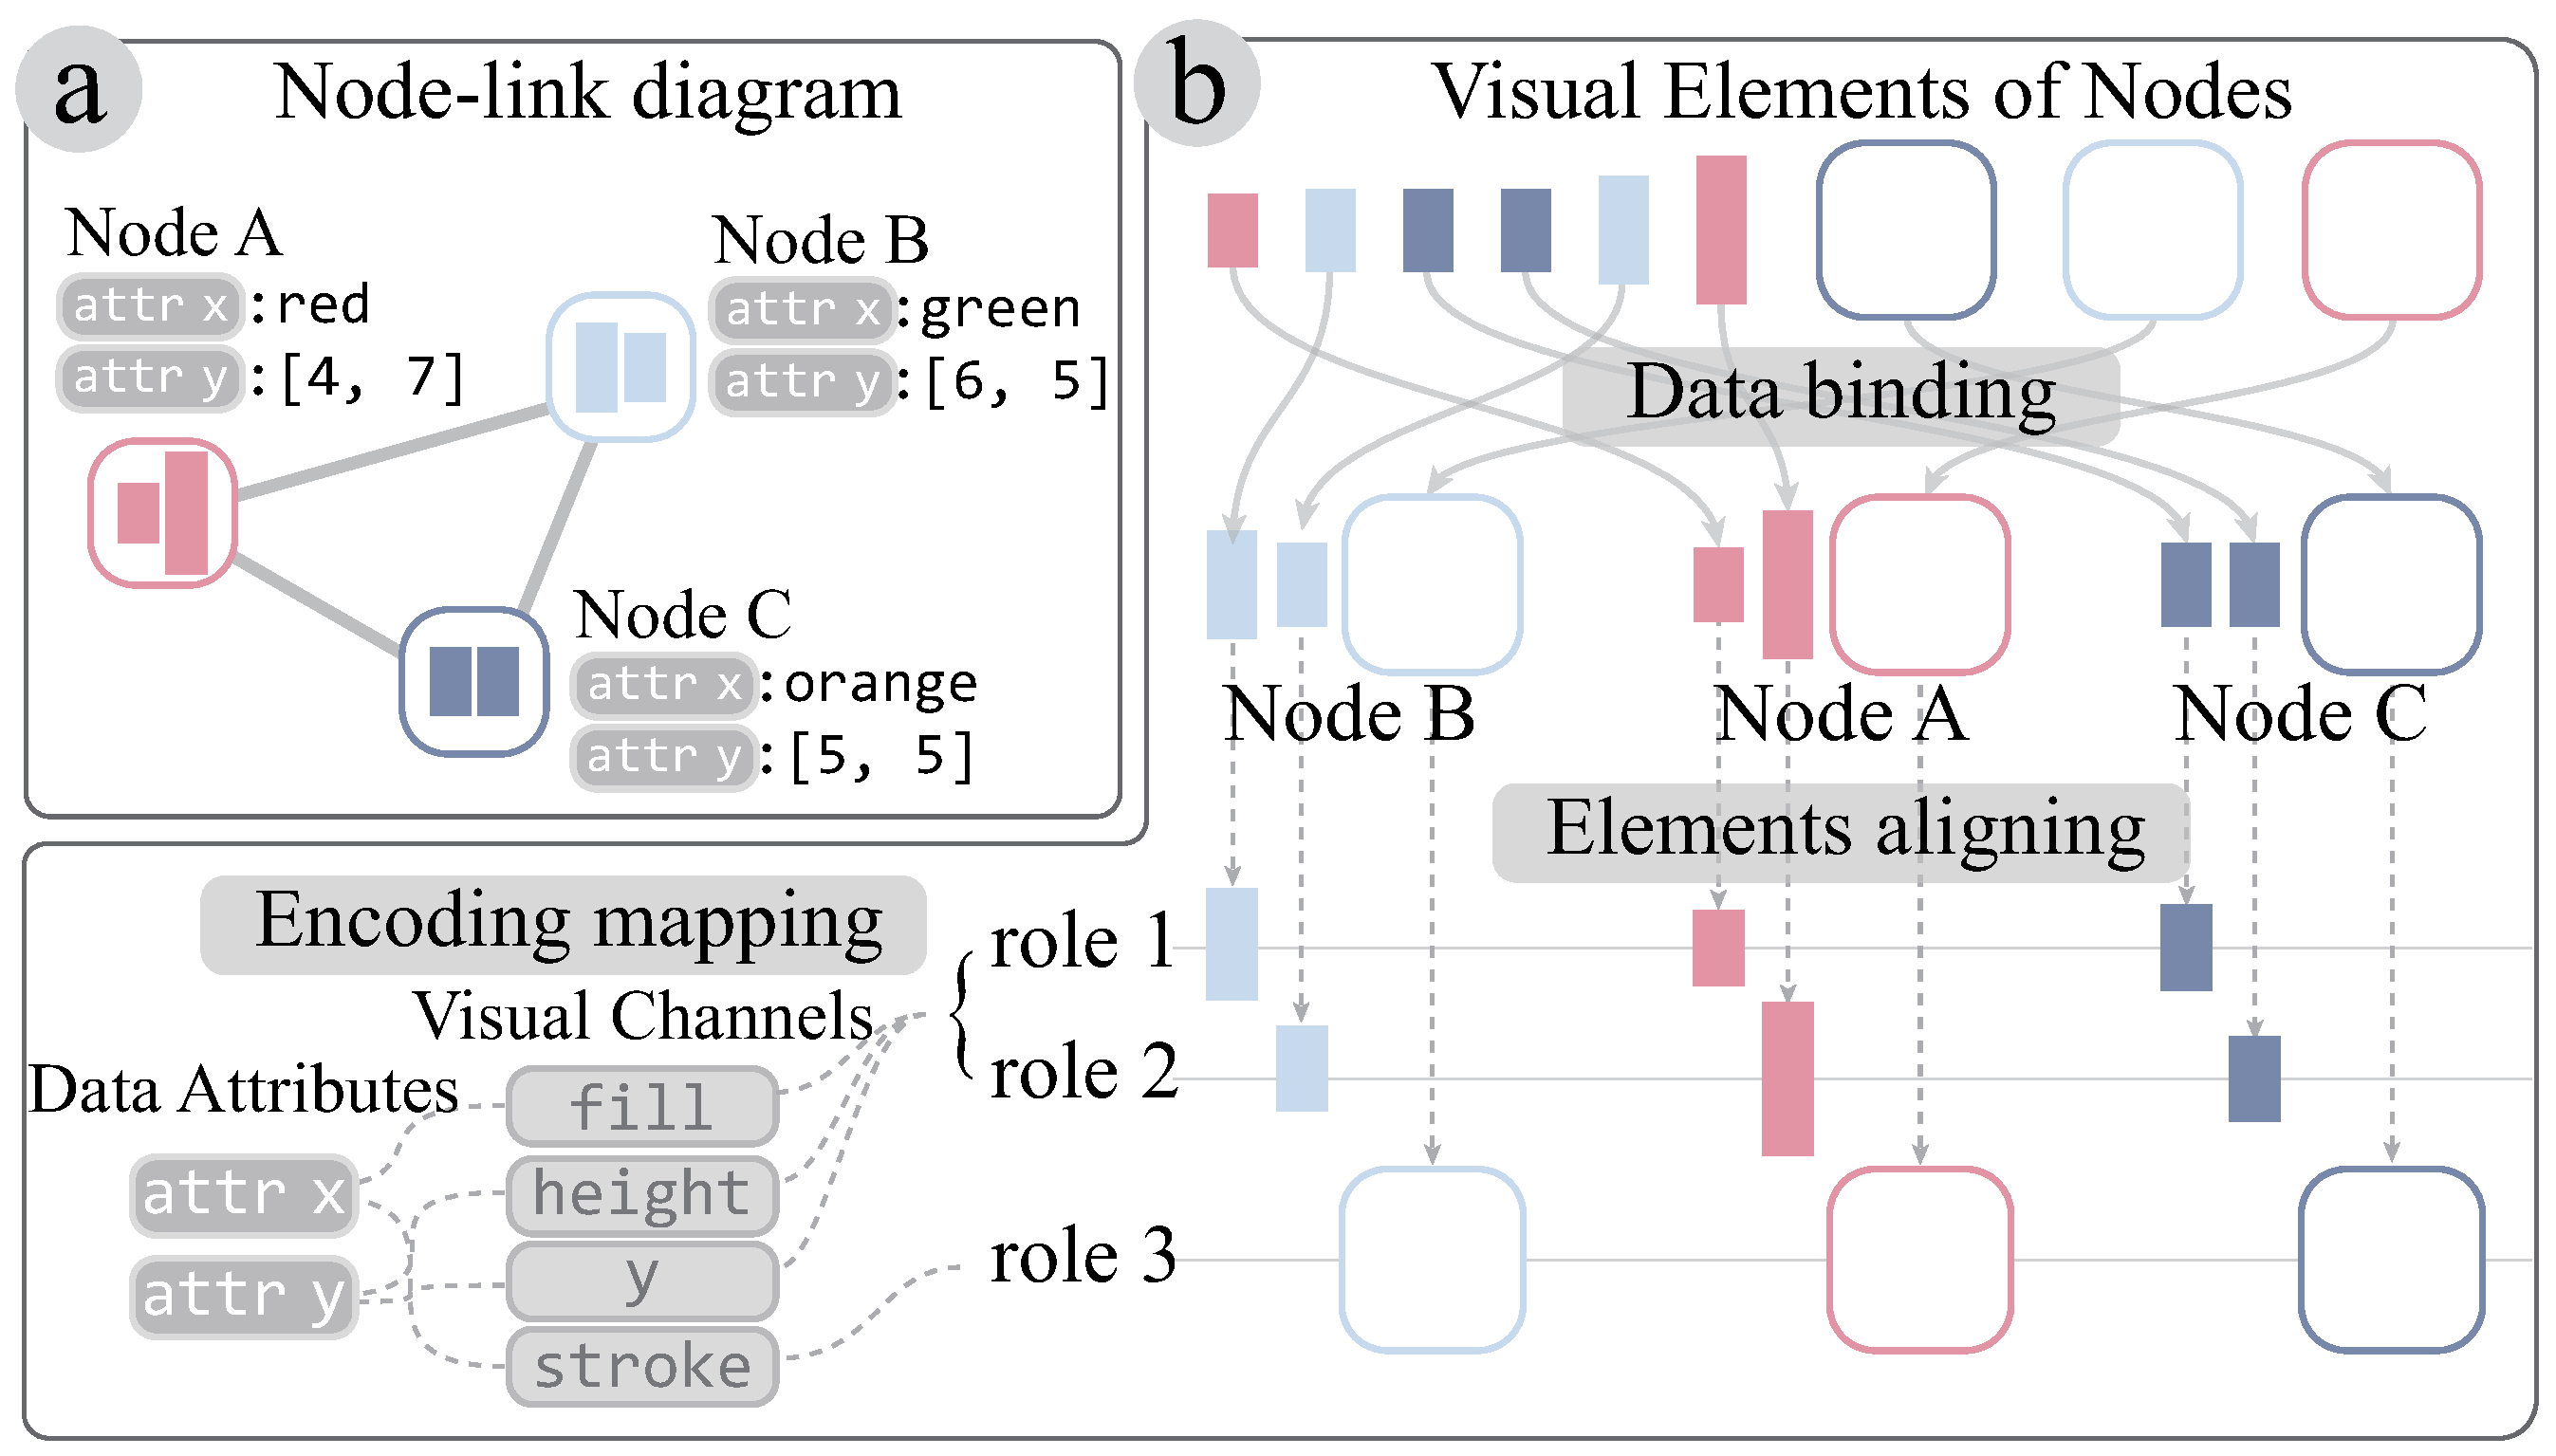
\includegraphics[width=1\columnwidth]{figures/VisualEncodings.eps}
    \caption{How \ApproachName~extracts visual encodings from a node-link diagram in the SVG format. A node-link diagram consists of three nodes and three links (upper left corner). Node elements are extracted and the \textbf {data binding} step maps them into different node entities. Then elements having the same role across different node entities are aligned into the same role class in the \textbf{elements aligning} step. Mappings among roles, visual channels, and attributes are detected by the \textbf{encoding mapping} step.}
    \label{fig:VisualEncodings}
\end{figure}

% 我们的工作通过分析源代码,从中提取数据实体()是如何被编码为视觉通道的()
We formulate the problem of describing visual encodings in node-link diagrams by three questions:
\begin{compactenum}[\textbf{Q}1]
    \item \textit{What elements does a node/link consist of in the diagram?} 
    For example, in Figure~\ref{fig:VisualEncodings}, a node is composed of three rectangles. \label{qstn:composition}
    
    \item \textit{What attributes do elements and their visual channels encode?} 
    For example, in Figure~\ref{fig:VisualEncodings}, the left rectangle's height in Node A encodes the first item of the attribute $y$. 
    % When the shape (\texttt{tagName}) of an element encodes some attribute, we should classify and discuss when elements are visualized as different shapes. 
    Attributes may be visualized in different ways according to the shape of the elements, such as the width and height of the \texttt{<rect>} and the radius of the \texttt{<circle>}.\label{qstn:encodings}
    % For example, when the node is encoded into a \texttt{<circle>}, the radius encodes its degree, and when the node is encoded into a \texttt{<rect>}, the width and the height encode its degree. 
    
    \item \textit{Is there a certain type of correlation (positive, negative, or categorical) between attributes and visual channels?}
    For example, the greater the degree of the node, the greater the radius of the circle.\label{qstn:correlation}
\end{compactenum}
Thus, it is necessary to extract mappings between \textbf{\textit{data entities}} and \textbf{\textit{visual elements}} and making correlations between \textbf{\textit{attributes}} and \textbf{\textit{visual channels}} to formulate the encoding scheme.

We define the encoding scheme as:
\begin{equation}
encoding := (entity, attribute, element, channel).
\end{equation}
Our target is to identify the entire set of encodings (Figure~\ref{fig:ElementAligning} (a)).

\begin{figure}[ht]
    \centering
    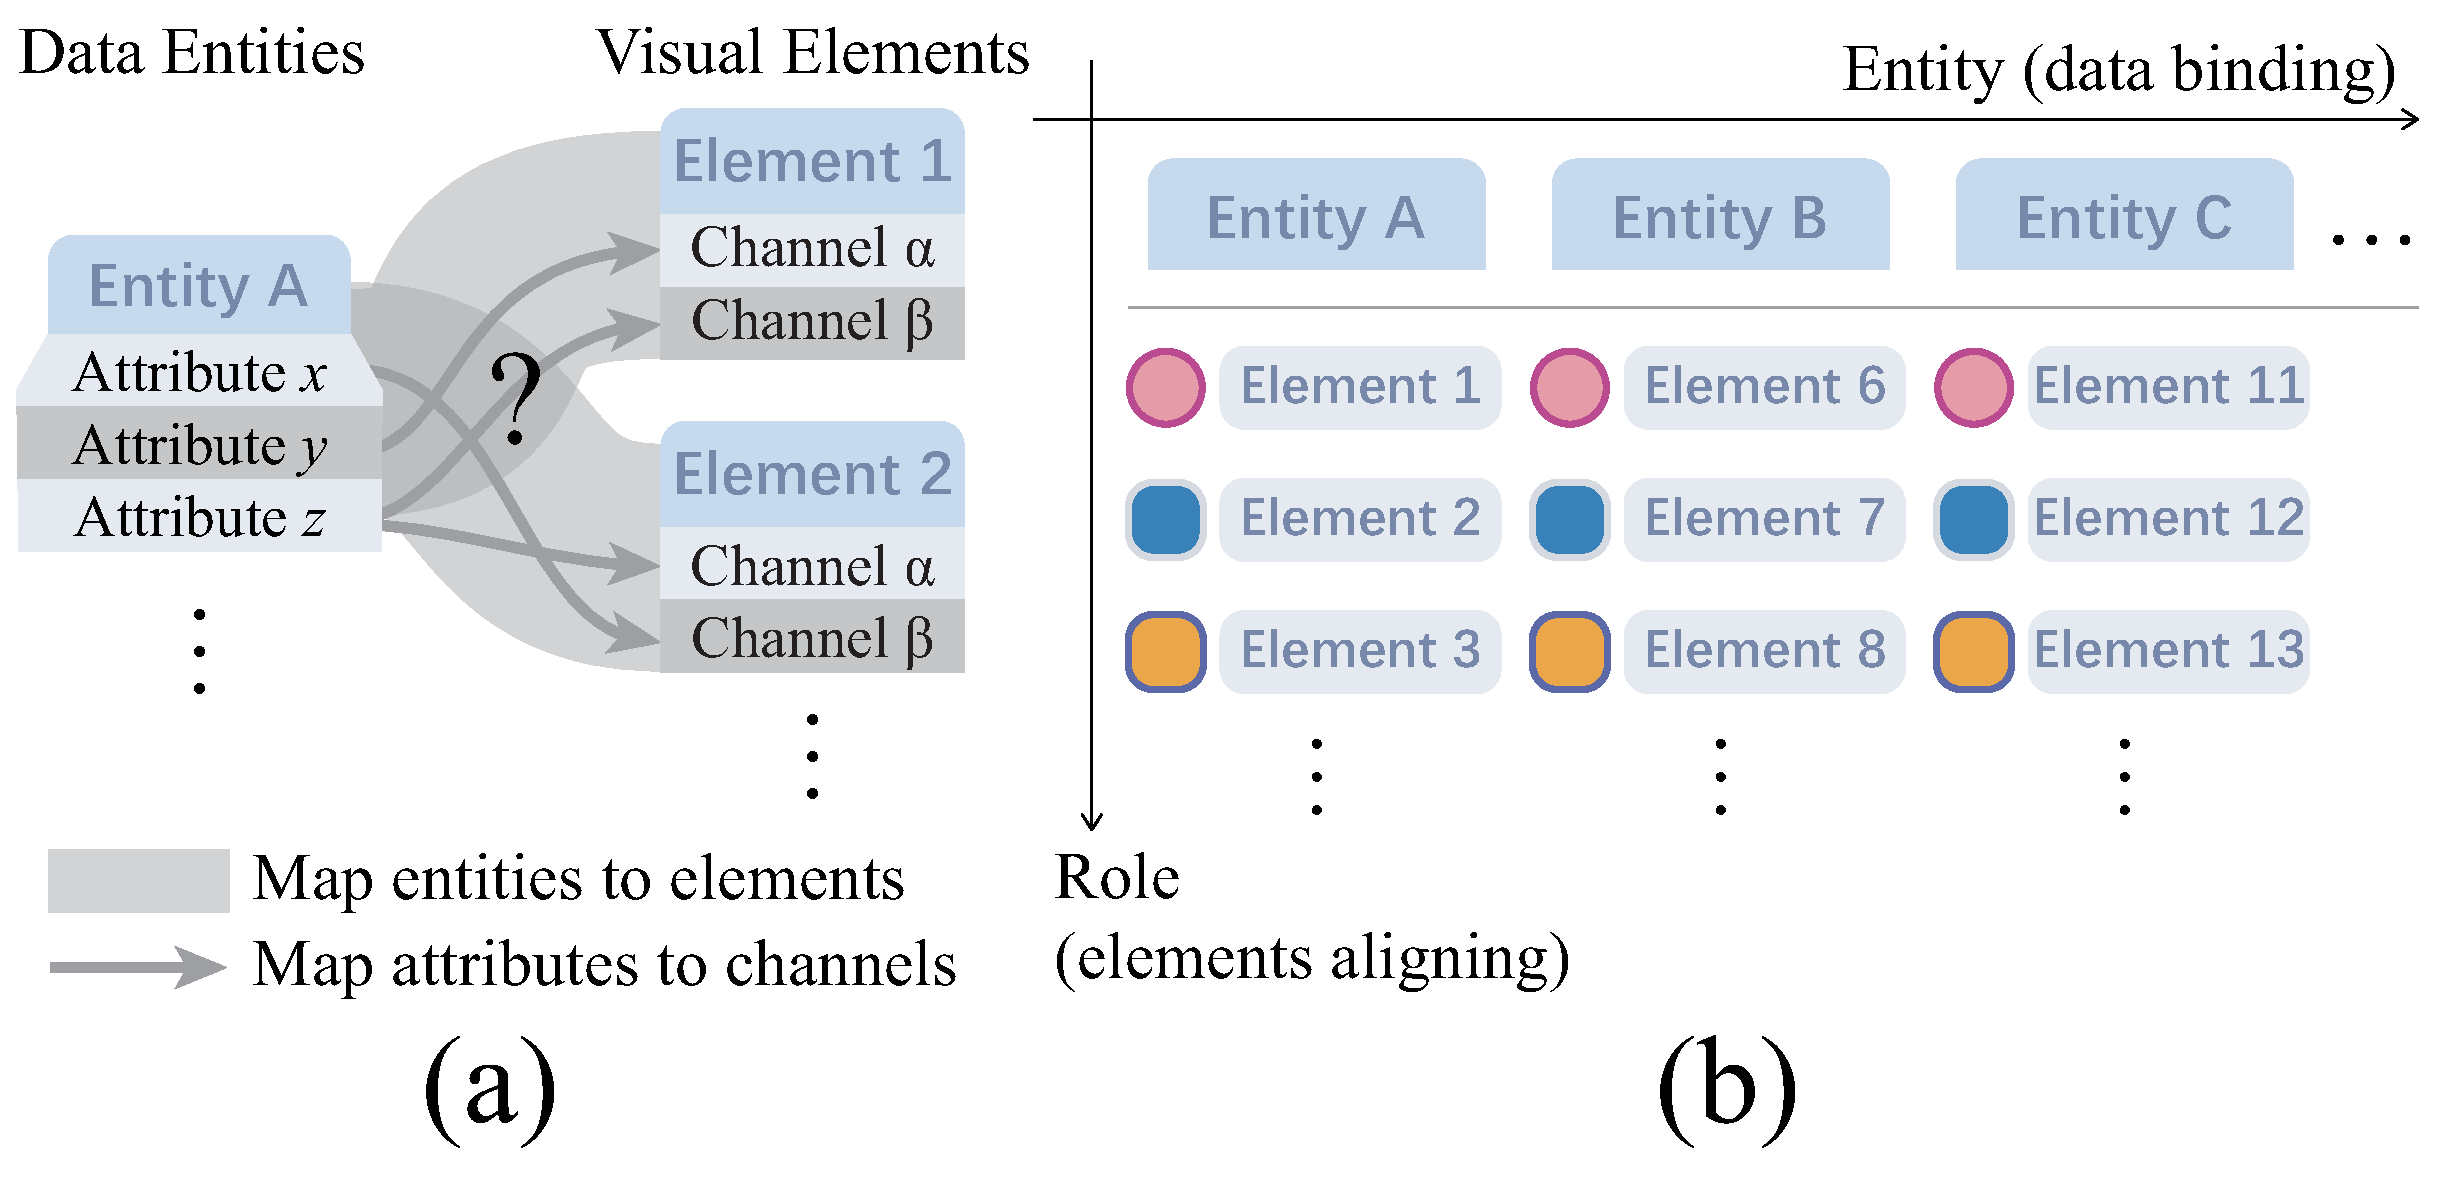
\includegraphics[width=1\columnwidth]{figures/ElementAligning.eps}
    \caption{(a) The target of our visual encoding detection technique; and (b) effect of the data-binding step and the elements-aligning step.}
    \label{fig:ElementAligning}
\end{figure}

% xxxx 等人的工作为我们提供了一个良好的思路,但他们的工作存在一些限制
A tool proposed by Harper and Agrawala~\cite{DBLP:conf/uist/HarperA14} provides a creative perspective for visual encoding extraction.
Although that tool can be extended to support simple node-link diagrams (where each data entity is encoded as only one element), several limitations exist:
\begin{compactenum}
% 1. 其需要创作者使用d3的数据绑定,才能发挥__data__的作用;使用其他工具,或者未将数据绑定到元素上时则无法使用该方法;
\item The D3's data-binding feature is required within the tool so by the ``\texttt{\_\_data\_\_}'' attribute of visual elements can be acquired. 
It cannot deal with general SVG-format visualizations without data bound to visual elements.

% 2. 其只能检验属性和视觉通道之间是否存在线性映射或者类别性映射。
\item It only supports the linear mapping and the categorical mapping and cannot maintain situations with complex visual mappings.
\end{compactenum}
These obstacles prevent it from extracting visual encodings from node-link diagrams created in the general SVG format.

% 我们针对节点链接图的场景,提出了一个数据绑定的策略,通过不断调整输入的数据,检查输出的变化,从而获取数据到svg元素之间的映射关系以及属性到视觉通道之间的映射方式,以解决以上两个问题。
For node-link diagrams, we introduce a new technique to solve such limitations.
Our technique incorporates the source code and the underlying graph data.
The key idea is regarding the source code as a black box.
Our technique modifies the input graph data and detects changes in the output SVG to obtain mappings between data entities and visual elements.
It overcomes the limitations by three steps (Figure~\ref{fig:VisualEncodings}):
(1) \textbf{Data binding} binds elements to different data entities.
(2) \textbf{Elements aligning} aligns elements according to their \textit{roles}. 
(3) \textbf{Encoding mapping} detects correlations among attributes, elements, and visual channels.

\subsection{Data Binding} \label{sec:databinding}
To detect mappings between \textbf{\textit{data entities}} and \textbf{\textit{visual elements}}, 
we modify attribute values of data entities and record corresponding visual element changes so as to construct mappings between the modified entity and the changed elements.
However, directly modifying attributes may deform the attribute distribution, and this can influence visual mappings so that elements related to other data entities may also be changed.
% 节点的size属性线性映射到编码该节点的圆形的半径r上,r[i] = (size[i] - min(size)) / (max(size) - min(size)) * max_radius
For example, the node's \texttt{size} attribute is linearly mapped into the radius of the \texttt{<circle>} element encoding the node: 
% $$radius_i = \frac{size_i - min(size)}{max(size) - min(size)} * radius_{max}$$
$radius_i = (size_i - min(size)) / (max(size) - min(size)) * radius_{max}$.
Modifying $size_i$ may broaden the attribute range and changes the linear mapping defined by the attribute range.
We prevent this by merely swapping attributes of two entities rather than modifying them, so that no new data is introduced and the distribution is preserved.
We take nodes as an example.
After swapping all two nodes' attributes, visual elements that differ from the previous are regarded as two nodes' corresponding elements.
For example, after swapping nodes B and C in Figure~\ref{fig:DataBinding} (b), elements 1 to 4 are changed.
All these changed elements correspond to nodes B and C because only B and C are swapped.
After swapping the node B with the node A in Figure~\ref{fig:DataBinding} (c), elements 2 and 3 are changed twice (Figure~\ref{fig:DataBinding} (b) and (c)), thus they correspond to node B because only node B are swapped twice.
% To ensure all elements of node B are detected, we swap it with all the other nodes.
Each node will be swapped with all other nodes to ensure that all elements belonging to it are detected.
After swapping all nodes, the entire node-to-element mapping is constructed (Figure~\ref{fig:DataBinding} (d)).
Node entities are bound to their corresponding elements.
The link-to-element mapping is constructed in the same way.
Because swapping two nodes may influence their related links, node-related elements can contain elements corresponding to links.
We remove elements corresponding to links from the node-to-element mappings.
Two parts ($entity$ and $element$) of the mapping relationship are solved.

\begin{figure}
    \centering
    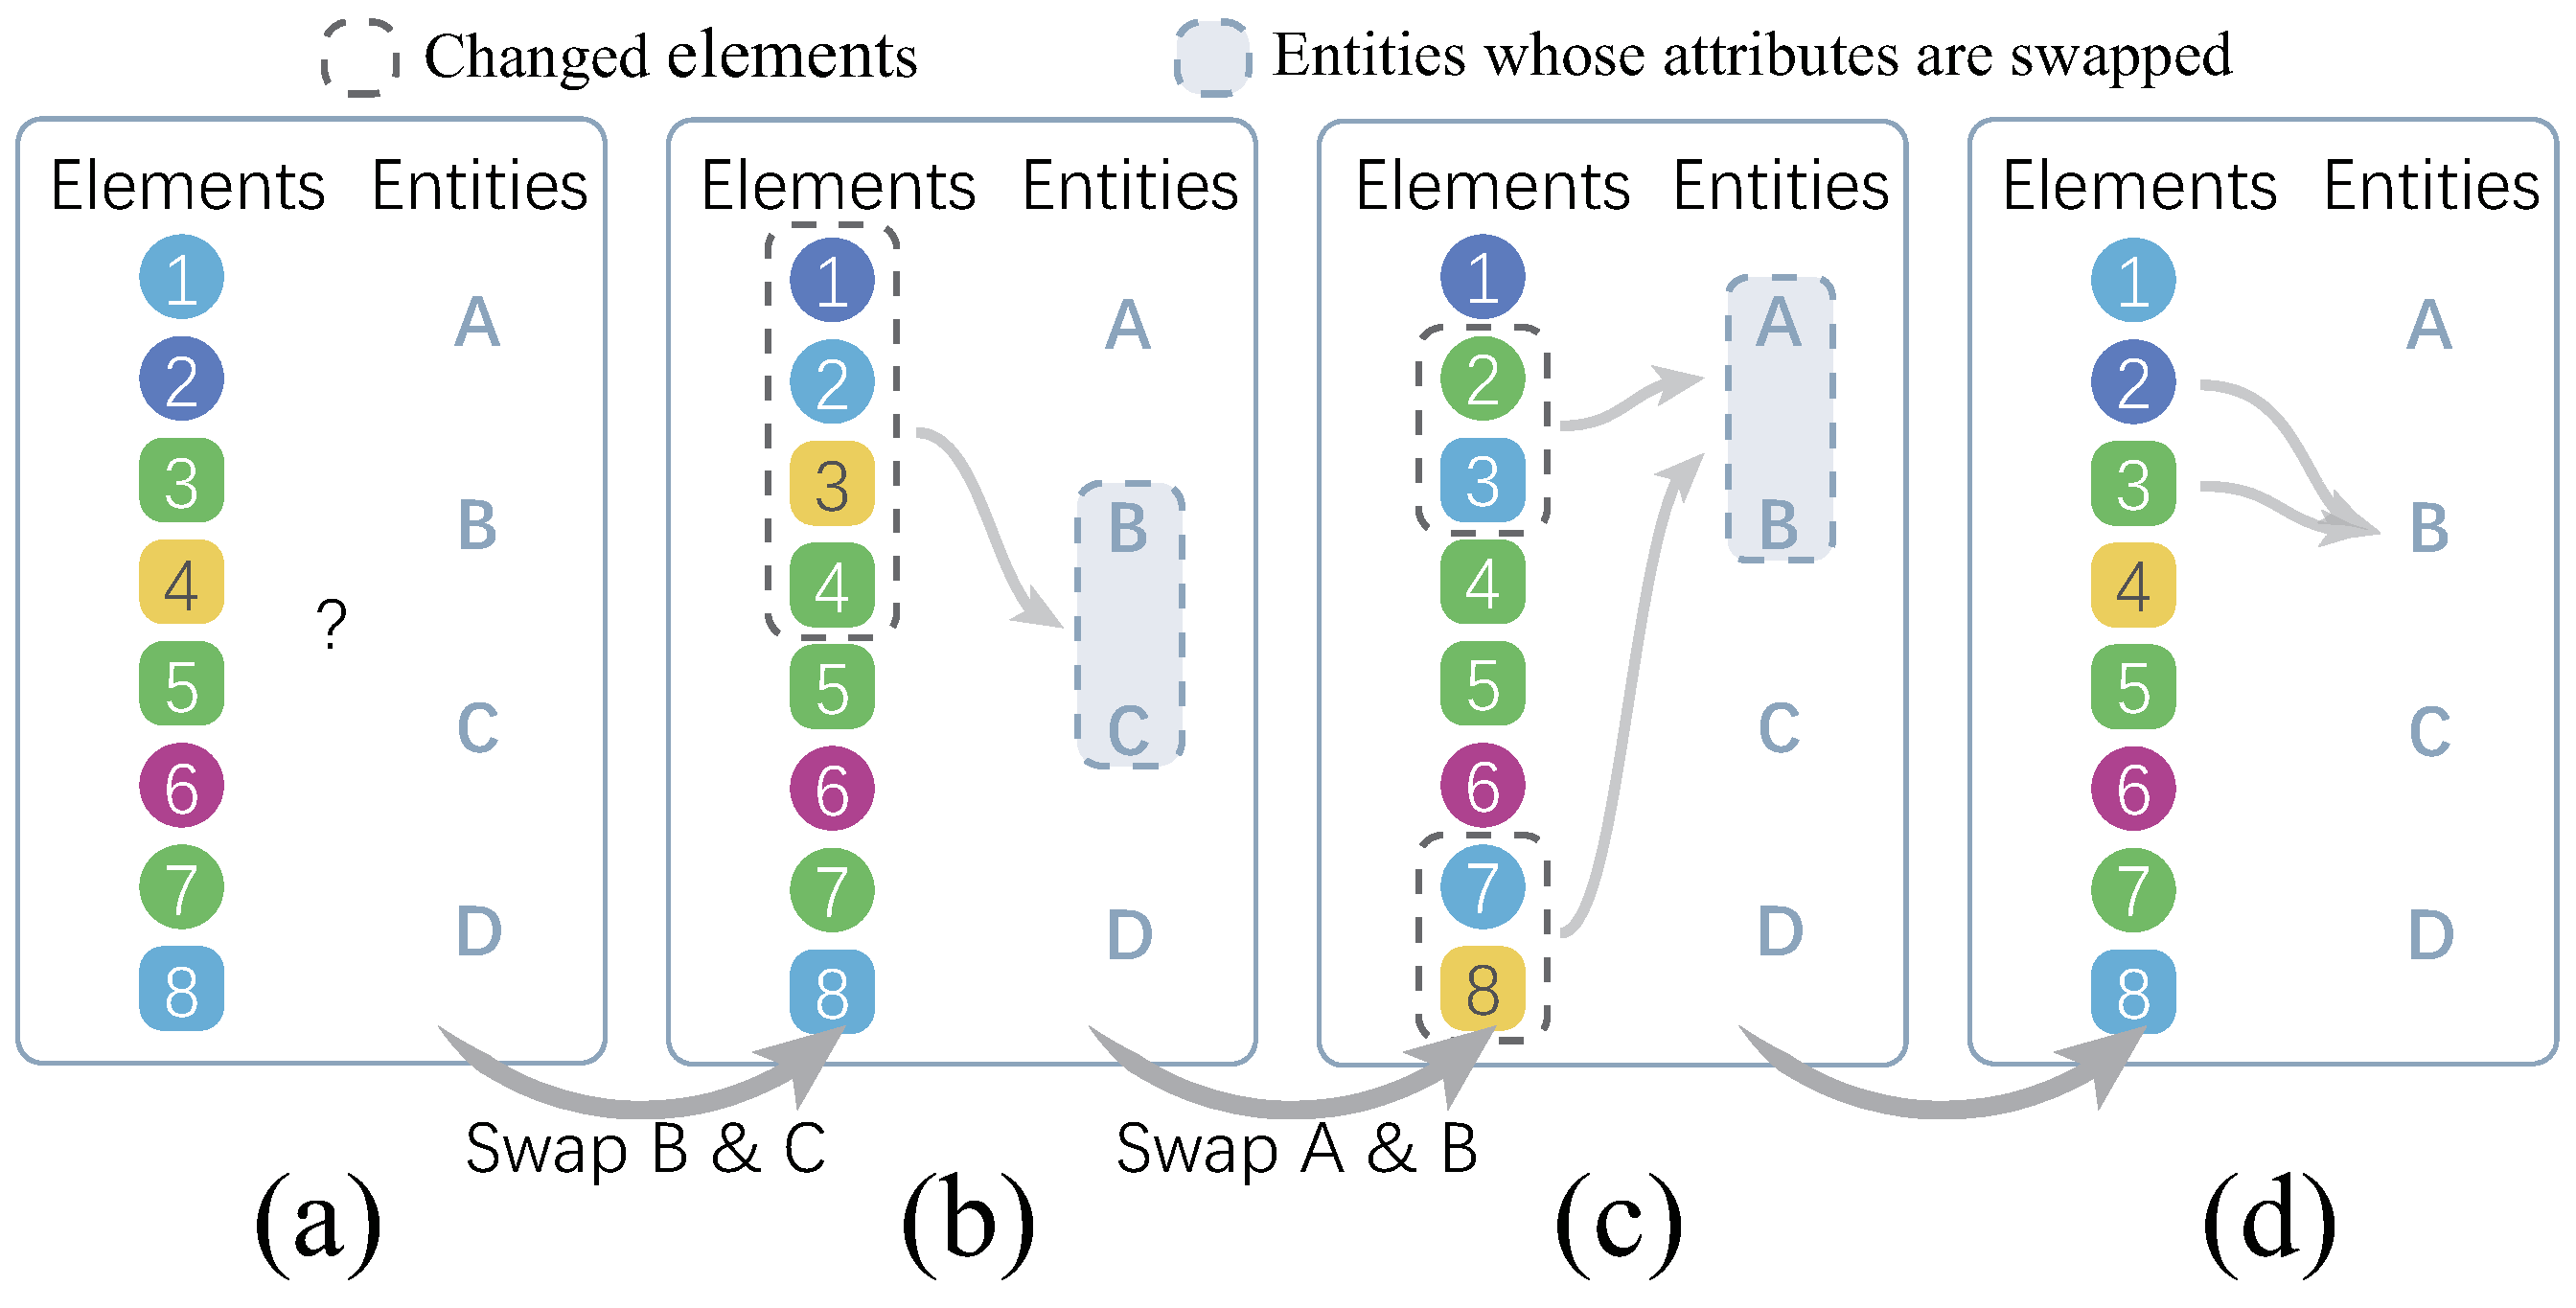
\includegraphics[width=1\columnwidth]{figures/DataBinding.eps}
    \caption{Data binding is achieved by swapping attributes of data entities. (a) Visual mappings between original visual elements and data entities are unknown. (b) After swapping attributes of entities B and C, the appearance of elements 1 to 4 is changed. Thus, entities B and C correspond to elements 1 to 4. (c) After swapping attributes of entities A and B, the appearance of elements 2, 3, 7, and 8 is changed. Thus, entities A and B correspond to these elements. (d) After swapping B with A and C, elements 2 and 3 change twice. We can map entity B to elements 2 and 3.}
    \label{fig:DataBinding}
\end{figure}

\subsection{Elements Aligning}
The data-binding step only binds visual elements into different data entities (the horizontal direction in Figure~\ref{fig:ElementAligning} (b)).
The roles of different elements are unknown.
The \textit{role} of an element is defined as a function that maps attributes to visual channels:
\begin{equation}
    role :=  \{attribute: value\} \mapsto \{channel: appearance\}
\end{equation}
% 两个元素相同角色,当且仅当,在它们所对应的数据实体的所有属性都相同时,它们的channels也都一样。
Two elements have the same role iff given arbitrary same inputs (all attributes of their corresponding entities), their outputs (all their visual channels) are the same.
For the example in Figure~\ref{fig:VisualEncodings}, 
roles of all three left inner rectangles are the same,
because if we swap all attributes of nodes A and B, node A's left rectangle before swapping will be same to node B's left rectangle after swapping regarding all their visual channels such as \texttt{x}, \texttt{y}, \texttt{fill}, and \texttt{height}.
They are aligned to classify their roles (the vertical direction in Figure~\ref{fig:ElementAligning} (b)).
% The \textit{role} can be regarded as a function that takes data attributes as input and assign values for visual element channels.
% Elements across different data entities are regarded as the same role if their effects are the same.
% Elements within the same role should appear exactly the same when their own nodes have exactly same attributes.
% 通过测试两个元素在同一属性输入时是否表现一致,来判断它们是否属于一种角色。
Different elements' role identity can be determined by swapping their corresponding data entities along with the data binding step, because all attributes of one entity before swapping are the same to the counterpart of the other one after swapping.
For example, in Figure~\ref{fig:DataBinding} (b), after swapping entity B with entity C, element 1 appear same to element 2 before swapping in Figure~\ref{fig:DataBinding} (a). Thus, elements 1 and 2 can be aligned into the same role.
We clarify the binding among visual elements, data attributes, and visual channels, which is conducive to the subsequent steps.
% 这样做的意义:能够使得数据和可视化之间的绑定更加清晰,有利于后续步骤的进行。


\subsection{Encoding mapping}\label{sec:encodingmapping}
The previous two steps classify elements according to two dimensions (the entity and the role) to solve \textbf{Q\ref{qstn:composition}}.
% 到此为止,我们已经已经知道每个实体是由哪些不同角色的元素组成,足够回答第一个问题
However, correlations between visual channels and data attributes are not determined.
% 我们继续以节点为例。
We continue to take nodes as an example.
% 为了检验一个属性究竟被编码在了哪些视觉通道上,我们通过shuffle所有节点的某个属性,观察视觉通道发生的变化。
We detect related visual channels of an attribute by shuffling all nodes' attributes and observing visual channel changes of their corresponding elements.
% 变化可以被定义为,某个属性引起某些元素的某些视觉通道的变化。
One correlation is defined as ``which \textit{attribute} changes which \textit{visual channel} of which \textit{element}''. We formalize it as:
\begin{equation}
    correlation := ( attribute, element, channel )
\end{equation}
% 然后我们根据不同的element角色,对这些发生的变化进行合并。
We merge different correlations according to the role of elements.
Thus, we replace the $element$ in the correlation's definition with $role$.
We obtain the entire correlation set of different roles to solve \textbf{Q\ref{qstn:encodings}}.
% It generates more comprehensive mappings between attributes and visual channels for elements of different roles.

Moreover, we identify the category of correlations to solve \textbf{Q\ref{qstn:correlation}}.
It requires the classification of attribute types and channel types.
We support numerical attributes and categorical attributes in \ApproachName.
List attributes and dictionary attributes are separated into multiple numerical attributes or categorical attributes (e.g.,\texttt{[1, 2, 3]}, \texttt{\{"year":2021,"month":03\}}).
We regard all visual channels as numerical (colors can be divided into RGB channels which are numerical).
However, numerical data can be used as categorical data if there are only a few classes of values.
For example, natural numbers are often used as categorical attributes such as labels, groups, and classes.
Thus, for numerical data, we must compare the number of unique values and their entries to determine whether it is numerical or categorical.
We set up a parameter $\alpha$ to make the distinction: if all values of the attribute are natural numbers and
the number of an attribute's unique values is less than $\alpha$ percent of the number of data entities, we regard the attribute as categorical.
% 我们根据属性和通道的类型来定义关系的类型
We identify the type of correlation by the type of attribute and channel:
\begin{compactitem}
    \item \textbf{The channel and attribute are categorical} or \textbf{the channel is categorical while the attribute is numerical}. 
    % 为了描述不同的channel取值所代表的的含义。我们为每类不同的channel记录了它们所对应的属性的取值范围。
    In order to describe the meanings of different channel values,
    We record the value range of the attribute for each category of channel values.
    % 假如在这种关系下,不同类别的channel对应的属性取值有交叉,我们则会抛弃这种关系,因为它具有歧义。
    If the attribute values corresponding to different channel values intersect, we discard this correlation because it is ambiguous.
    
    \item \textbf{The channel and attribute are numerical}. We compute the Pearson's Correlation Coefficient and test whether the correlation is positive, negative, or uncorrelated with the coefficient and the significance test's p-value. We take the attribute as a factor that influences the visual channel when the absolute value of the coefficient is larger than $\theta$, and the $p$-value of the significance test is less than $\alpha$. We set $\theta = 0.5$ and $\alpha = 0.05$ by default, both parameters can be adjusted on-demand.
\end{compactitem}
The correlation type where \textbf{the channel is numerical while the attribute is categorical} is not supported because it is counterintuitive.




%********************* VERSION BEFORE 2021/04/01 *********************%
\iffalse
% % 我们提出了xxx,通过抽取信息并填充模板的方式来描述节点链接图,它大概分为三个步骤~\REf{}:1. xxx; xxx
% We introduce \ApproachName, which describes node-link diagrams by extracting information and filling templates.
None of these approaches is tailored for generating descriptions for node-link diagrams. 
We propose an approach named \ApproachName~to generate descriptions for node-link diagrams automatically.
It utilizes three information extraction pipelines to detect crucial information from the source code and the underlying graph and generates template-based descriptions.
The pipeline of \ApproachName~consists of three steps (Figure~\ref{fig:workflow}), which interprets:
\textbf{1) linking conditions} to describe how nodes relationships are constructed by finding, filtering, and sorting conditions;
\textbf{2) visual encodings} by extracting visual mappings among data entities, attributes, visual elements, and visual channels; and
\textbf{3) layout intention} by identifying different kinds of layouts and their affecting factors.

We implement an interactive interface based on \ApproachName, in which creators can input the source code and data to generate node-link diagrams and descriptions.
We augment the generated descriptions by highlighting interactions to enhance understanding.
When audiences hover on sentences of descriptions, relevant parts of the diagram are highlighted.

\begin{figure}
    \centering
    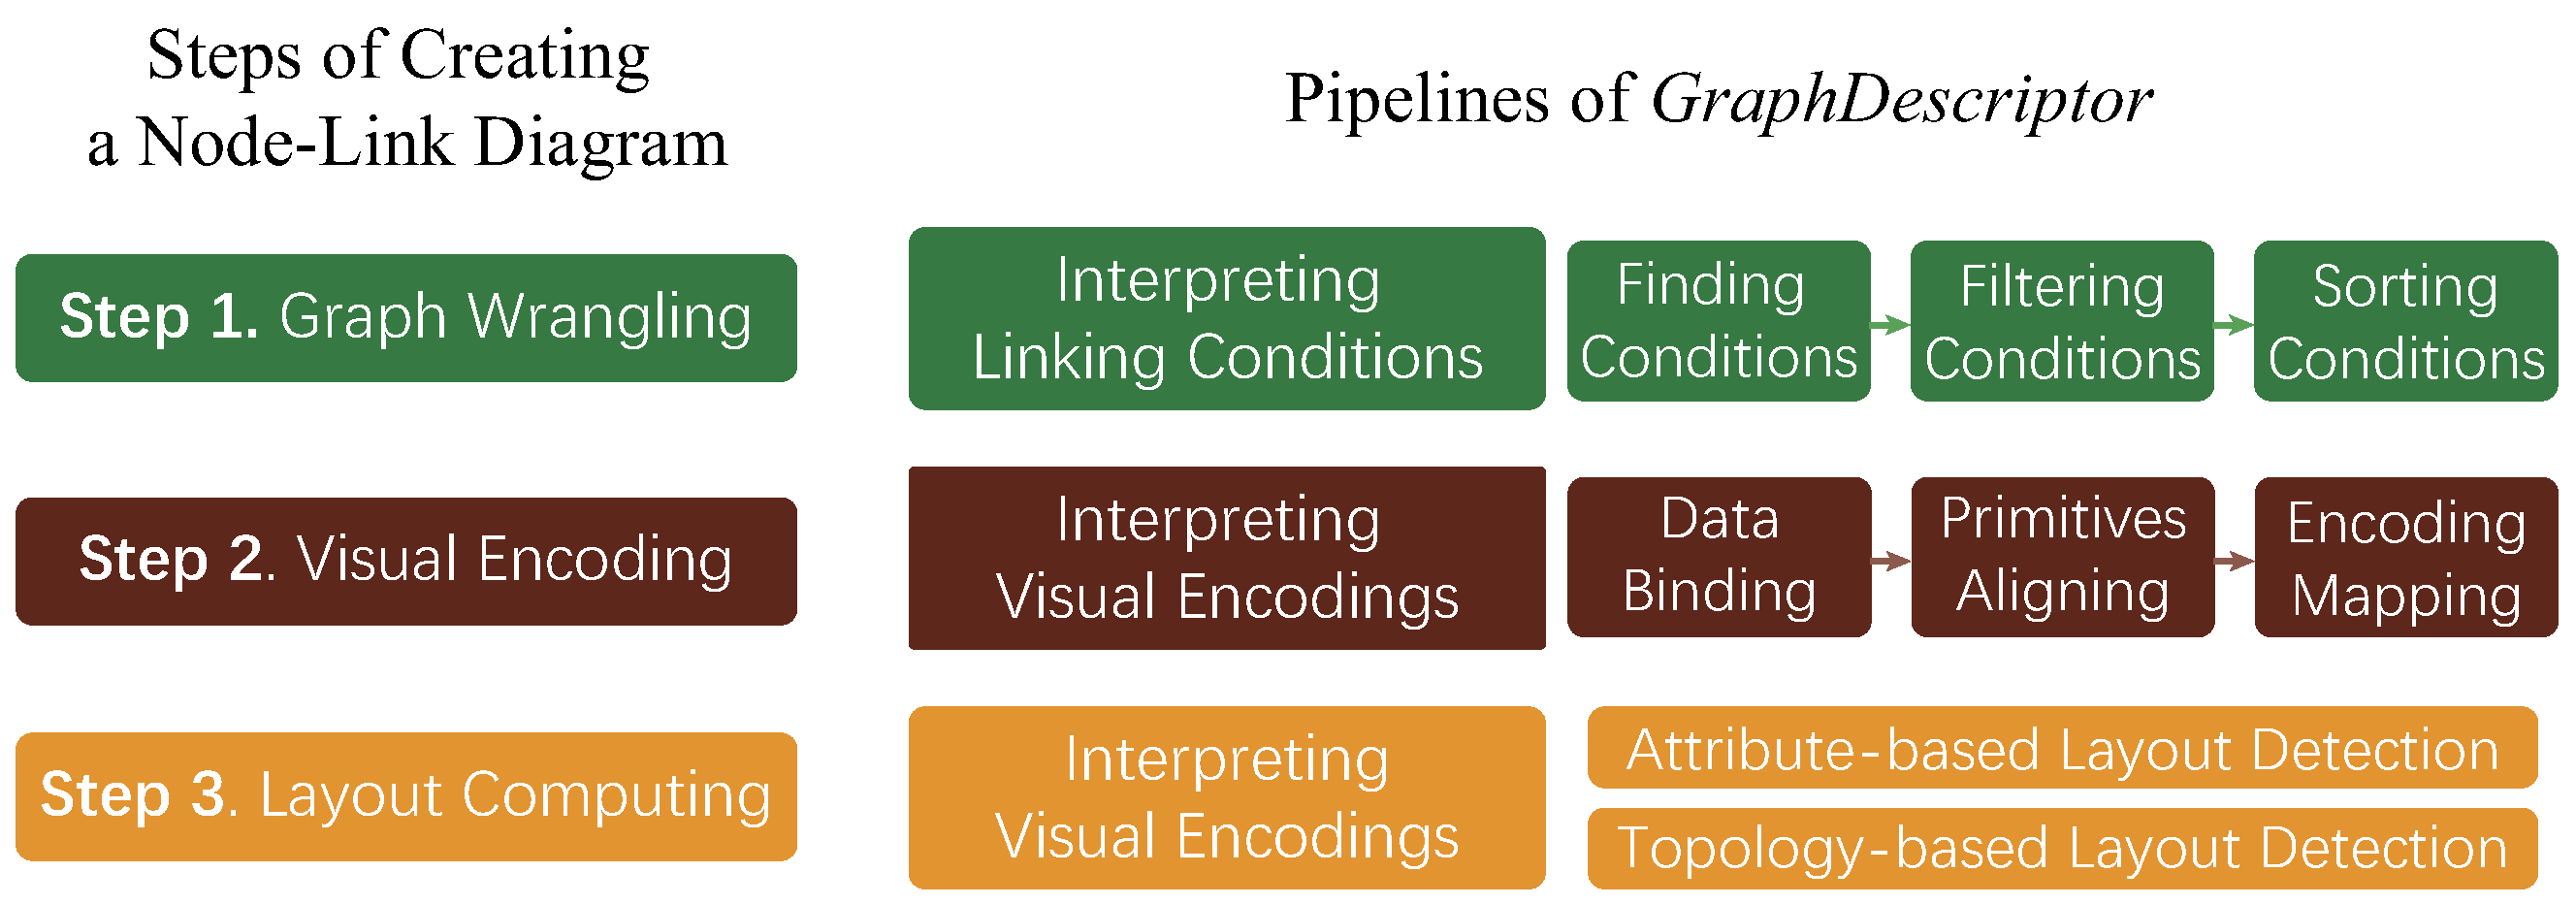
\includegraphics[width=1\columnwidth]{figures/workflow.eps}
    \caption{The pipeline of \textit{\ApproachName} follows the three-step creation process of node-link diagrams to interpret linking conditions, visual encodings, and layout intention.}
    \label{fig:workflow}
\end{figure}


\subsection{Interpreting Linking Conditions}
% 从表格型数据创建图数据时,最重要的就是建立节点之间的关系。
% 观众从节点链接图中所能获知的信息仅仅是某两个节点之间存在联系,但却不了解联系的内在含义。
% 一些论文已经对可能建立链接的情况进行了定义,
Several techniques~\cite{DBLP:journals/ivs/LiuNS14, DBLP:journals/ivs/HeerP14, DBLP:journals/tvcg/SrinivasanPEB18} of graph wrangling identify link construction as the crucial process and propose several linking conditions.
Thus our technique describes linking conditions to interpret the graph wrangling step.
Ploceus~\cite{DBLP:journals/ivs/LiuNS14} and Orion~\cite{DBLP:journals/ivs/HeerP14} infer potential linking conditions by constructing a linking graph and searching valid linking paths. They construct links among multiple data tables by analyzing primary and foreign keys.
Graphiti
Graphiti~\cite{DBLP:journals/tvcg/SrinivasanPEB18} identifies potential linking conditions of a homogeneous graph by comparing different attributes.
% 如果多个表合并成一个表,前两者总结的条件可以被Graphiti提出的规则所覆盖
Because multiple tables can be merged into one data table with primary and foreign keys, Graphiti can cover the linking conditions by identifying Ploceus's and Orion's rules.
Those works infer the potential linking conditions when only a few links are constructed;
% 我们尝试从它们的反方向进行思考,也就是,当我们获取到了所有的链接的时候,推测这些链接是如何被构建的
our method, on the other hand, works in the opposite direction from already constructed links.

\textbf{Finding Conditions}. We first construct conditions between all pairs of nodes. The conditions summarized by Graphiti can be organized into four categories:
\begin{compactenum}[\textbf{C}1]
    % 两个节点的某个属性值相同
    \item Values of an attribute of two nodes are the same, e.g., linking two movies published in the same year.
    % 两个节点的某个属性拥有超过一个共同的值
    \item Two nodes have at least one common value of a list attribute, e.g., linking two movies with one or more of the same actors.
    % 两个节点的某个属性值非常接近
    \item Values of an attribute of the two nodes are significantly close, where \textit{significance} is defined by the normalized difference.
    \item Values of an attribute of two nodes are in the same bin, where the bins are separated by quartiles.
\end{compactenum}

% 为了能够将这些condition填充到文本模板中,我们对condition的输出进行了formalize
We formalize the conditions with three aspects to facilitate comparison, sorting and filtering.
One condition can be defined as:
\begin{equation}
    linking\text{ }condition := ( type, attribute, value )
\end{equation}
where $type$ is the condition type, $attribute$ is the name of the attribute, $value$ is the value of the attribute when the condition holds.

\textbf{Filtering Conditions}.
We first detect linking conditions held on node pairs without any connections.
These conditions are regarded as false condition because no links exist, and should be filtered out.
Only conditions whose occurrences are no less than the number of links are selected from the rest conditions (Algorithm~\ref{alg:conditions}).

\textbf{Sorting Conditions}.
% After that, conditions are sorted by their \textit{degrees} and the highest-ranked condition will be regarded as the most possible condition.
% Degrees of conditions can be compared by their implication relations.
After that, conditions are sorted by their degrees through the comparison of their implication relations, the highest-ranked condition is regarded as the most likely condition.
For example, the condition $(type=C2, attribute=actors, value=[Alice, Bob])$ is implied by $(type=C2, attribute=actors, value=[Alice])$ and $(type=C2, attribute=actors, value=arbitrary\text{ }value)$, where $(value=arbitrary\text{ }value)$ means the condition does not assume the $actors$ attribute should equal to a certain value.
Its has a higher degree than the others, and is thus ranked higher.

We textualize the linking condition of the graph by filling templates. 
Four templates correspond to four conditions according to the $type$:
\begin{compactenum}[\textbf{T}1]
    \item \textit{``Two nodes are connected if the values of the attribute $@attribute$ are the same\$\{ ($@value$)?\}''}.
    \item \textit{``Two nodes are connected if the values of the attribute $@attribute$ have common values\$\{ ($@value$)?\}}''.
    \item \textit{``Two nodes are connected if the values of the attribute $@attribute$ are close (with a difference less than $@value$)''}.
    \item \textit{``Two nodes are connected if the values of the attribute $@attribute$ are within the same \$\{$@value$ ?\}bin''}.
\end{compactenum}
Here \$\{?\} means an included part that can be omitted and $@$ represents a placeholder.
For example, two movies sharing the same actors Alice and Bob are connected under the Condition \textbf{C2}, which could be represented as: $(type=C2, attribute=actors, value=[Alice, Bob])$. 
Its corresponding description is: \textit{``Two nodes are connected if the values of the attribute actors have common values ([Alice, Bob])''}. 
For the condition $(type=C2, attribute=actors, value=arbitrary\text{ }value)$, contents in its parentheses are omitted.

\begin{algorithm}[!t]
    \renewcommand\arraystretch{1.2}
    \caption{ Filtering Conditions }
    \label{alg:conditions}
    \begin{algorithmic}[1]
        \Require
            $G=(V=\{v_1, v_2, ..., v_n\}, E=\{e_1, e_2, ..., e_n\})$: a graph;
        \Ensure
            $C$: the potential condition set
        \State Init conditions $C=\varnothing$, false conditions $FC=\varnothing$
        \For {each node pair $(v_i, v_j)$}
            \If {$(v_i, v_j)$ is not a link}
                \State $C_{ij} \gets$ all conditions that can link $(v_i, v_j)$
                \State merge $FC$ with $C_{ij}$
            \EndIf
        \EndFor
        \For {each link $e_k=(v_i, v_j)$}
            \State $C_{ij} \gets$ all conditions that can construct link $e_i$
            \For {each condition $c$ in $C_{ij}$}
                \If {$c$ in $FC$}
                    \State remove $c$ from $C_{ij}$
                \EndIf
            \EndFor
            \State merge $C$ with $C_{ij}$
        \EndFor
        \For {each condition $c$ in the condition set $C$}
            \If {the frequency of $c$ is less than $|E|$}
                \State remove $c$ from $C$
            \EndIf
        \EndFor
        \State \Return $C$
    \end{algorithmic}
\end{algorithm}


\subsection{Interpreting Visual Encodings}\label{sec:visualencodings}
\subsubsection{Background}
% 为了在节点链接图中展示节点、链接的属性,常常将这些属性编码为节点/链接的视觉通道。
Creators often encode attributes of nodes and links by visual channels to reveal attribute-based patterns.
Nodes and links contained in the underlying graph are denoted as \textit{data entities} and each data entity consists of several \textit{attributes}.
For the node-link diagram example in Figure~\ref{fig:VisualEncodings}, a node contains a categorical attribute (\textit{x}) and a numerical list attribute (\textit{y}), We encode the list attribute \textit{y} with the height of two rectangles.
Then we encode the attribute \textit{x} with the two rectangles' fill color and the background rectangle's stroke color.

% 我们的方法处理的对象是基于SVG的。
\ApproachName~seeks to extract visual encodings from node-link diagrams in the SVG format, which is widely used in the visualization area.
Visualization creators can write programs with the W3C DOM API to construct visualizations within SVG.
A SVG includes a root element \texttt{<svg>} and allows hierarchical grouping of subelements with group elements \texttt{<g>}.
Marks onscreen are generated by graphical elements such as \texttt{<rect>}, \texttt{<circle>}, and \texttt{<ellipse>}.
We call these graphical elements \textit{visual elements}.
Their style attributes such as \texttt{cx}, \texttt{cy}, \texttt{width}, and \texttt{height} are denoted as \textit{visual channels}.
Each kind of visual elements has both unique channels (e.g., \texttt{width} and \texttt{height} are only owned by \texttt{<rect>}) and universal channels (e.g., \texttt{fill}, \texttt{stroke-width}).

\begin{figure}[ht]
    \centering
    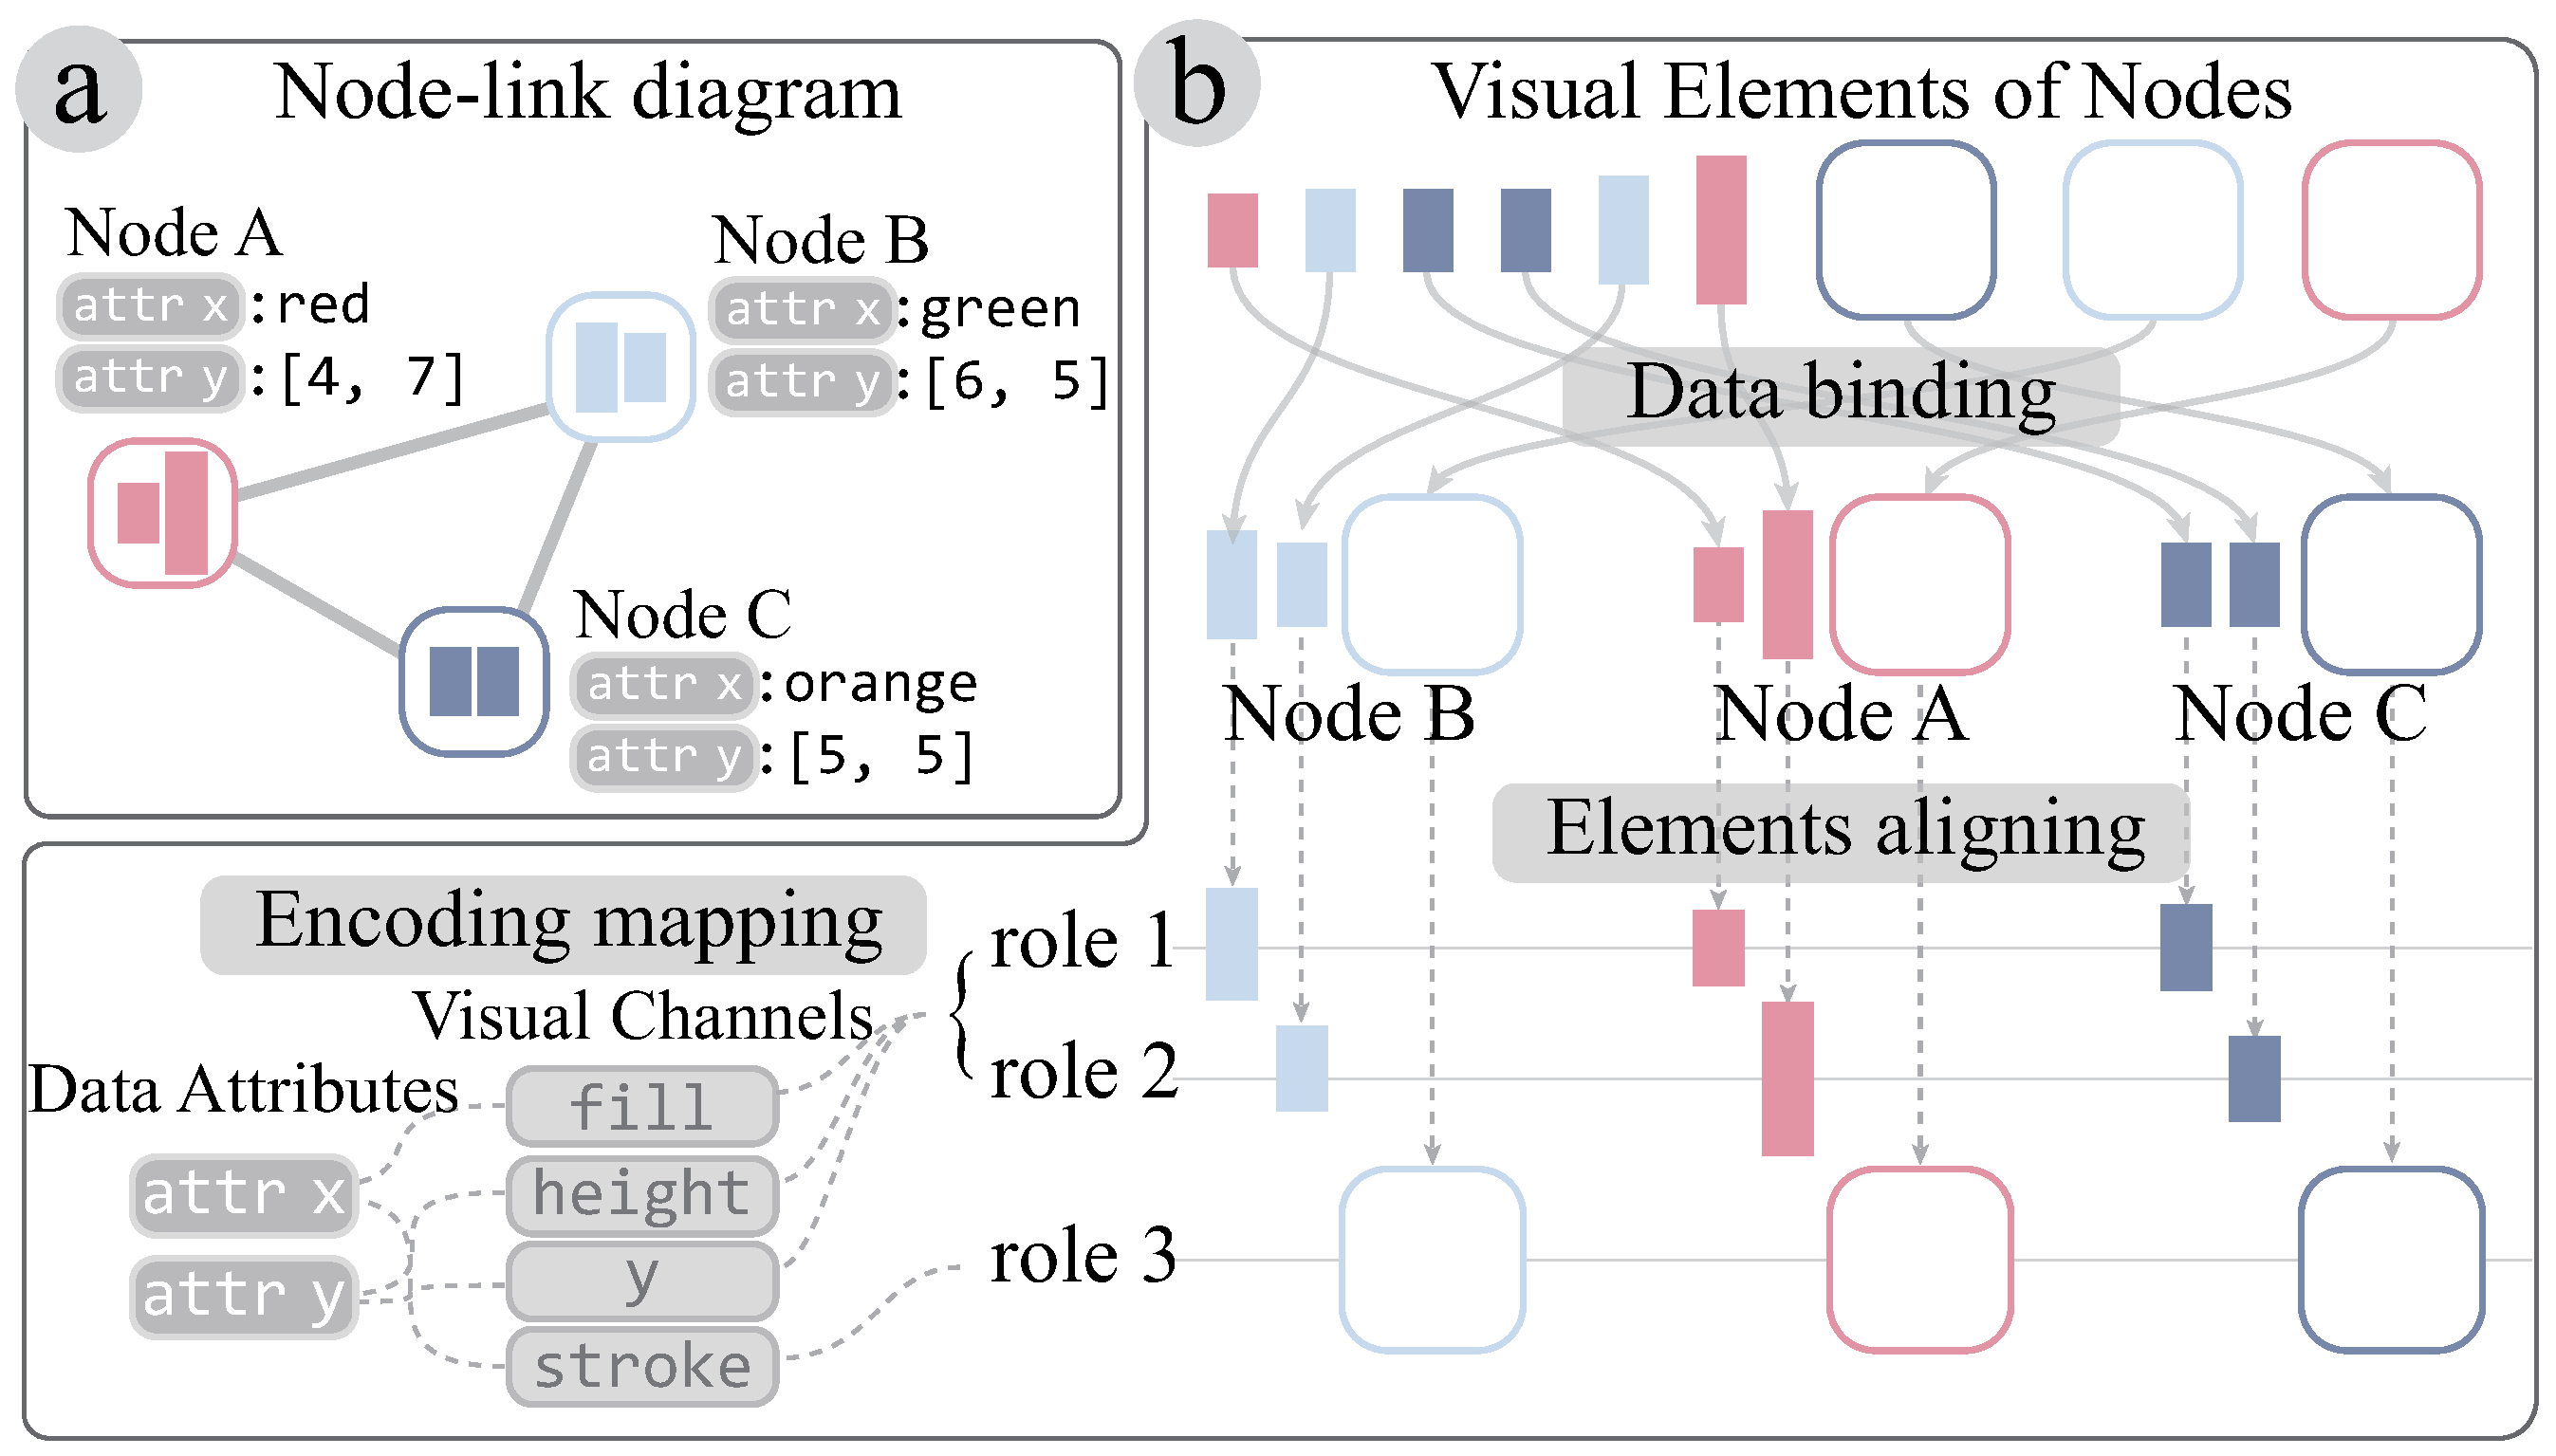
\includegraphics[width=1\columnwidth]{figures/VisualEncodings.eps}
    \caption{How \ApproachName~extracts visual encodings from a node-link diagram in the SVG format. A node-link diagram consists of three nodes and three links (upper left corner). Node elements are extracted and the \textbf {data binding} step maps them into different node entities. Then elements having the same role across different node entities are aligned into the same role class in the \textbf{elements aligning} step. Mappings among roles, visual channels, and attributes are detected by the \textbf{encoding mapping} step.}
    \label{fig:VisualEncodings}
\end{figure}

% 我们的工作通过分析源代码,从中提取数据实体()是如何被编码为视觉通道的()
We formulate the problem of describing visual encodings in node-link diagrams by three questions:
\begin{compactenum}[\textbf{Q}1]
    \item \textit{What elements does a node/link consist of in the diagram?} 
    For example, in Figure~\ref{fig:VisualEncodings}, a node is composed of three rectangles. \label{qstn:composition}
    
    \item \textit{What attributes do elements and their visual channels encode?} 
    For example, in Figure~\ref{fig:VisualEncodings}, the left rectangle's height in Node A encodes the first item of the attribute $y$. 
    % When the shape (\texttt{tagName}) of an element encodes some attribute, we should classify and discuss when elements are visualized as different shapes. 
    Attributes may be visualized in different ways according to the shape of the elements, such as the width and height of the \texttt{<rect>} and the radius of the \texttt{<circle>}.\label{qstn:encodings}
    % For example, when the node is encoded into a \texttt{<circle>}, the radius encodes its degree, and when the node is encoded into a \texttt{<rect>}, the width and the height encode its degree. 
    
    \item \textit{Is there a certain type of correlation (positive, negative, or categorical) between attributes and visual channels?}
    For example, the greater the degree of the node, the greater the radius of the circle.\label{qstn:correlation}
\end{compactenum}
Thus, it is necessary to extract mappings between \textbf{\textit{data entities}} and \textbf{\textit{visual elements}} and making correlations between \textbf{\textit{attributes}} and \textbf{\textit{visual channels}} to formulate the encoding scheme.

We define the encoding scheme as:
\begin{equation}
encoding := (entity, attribute, element, channel).
\end{equation}
Our target is to identify the entire set of encodings (Figure~\ref{fig:ElementAligning} (a)).

\begin{figure}[ht]
    \centering
    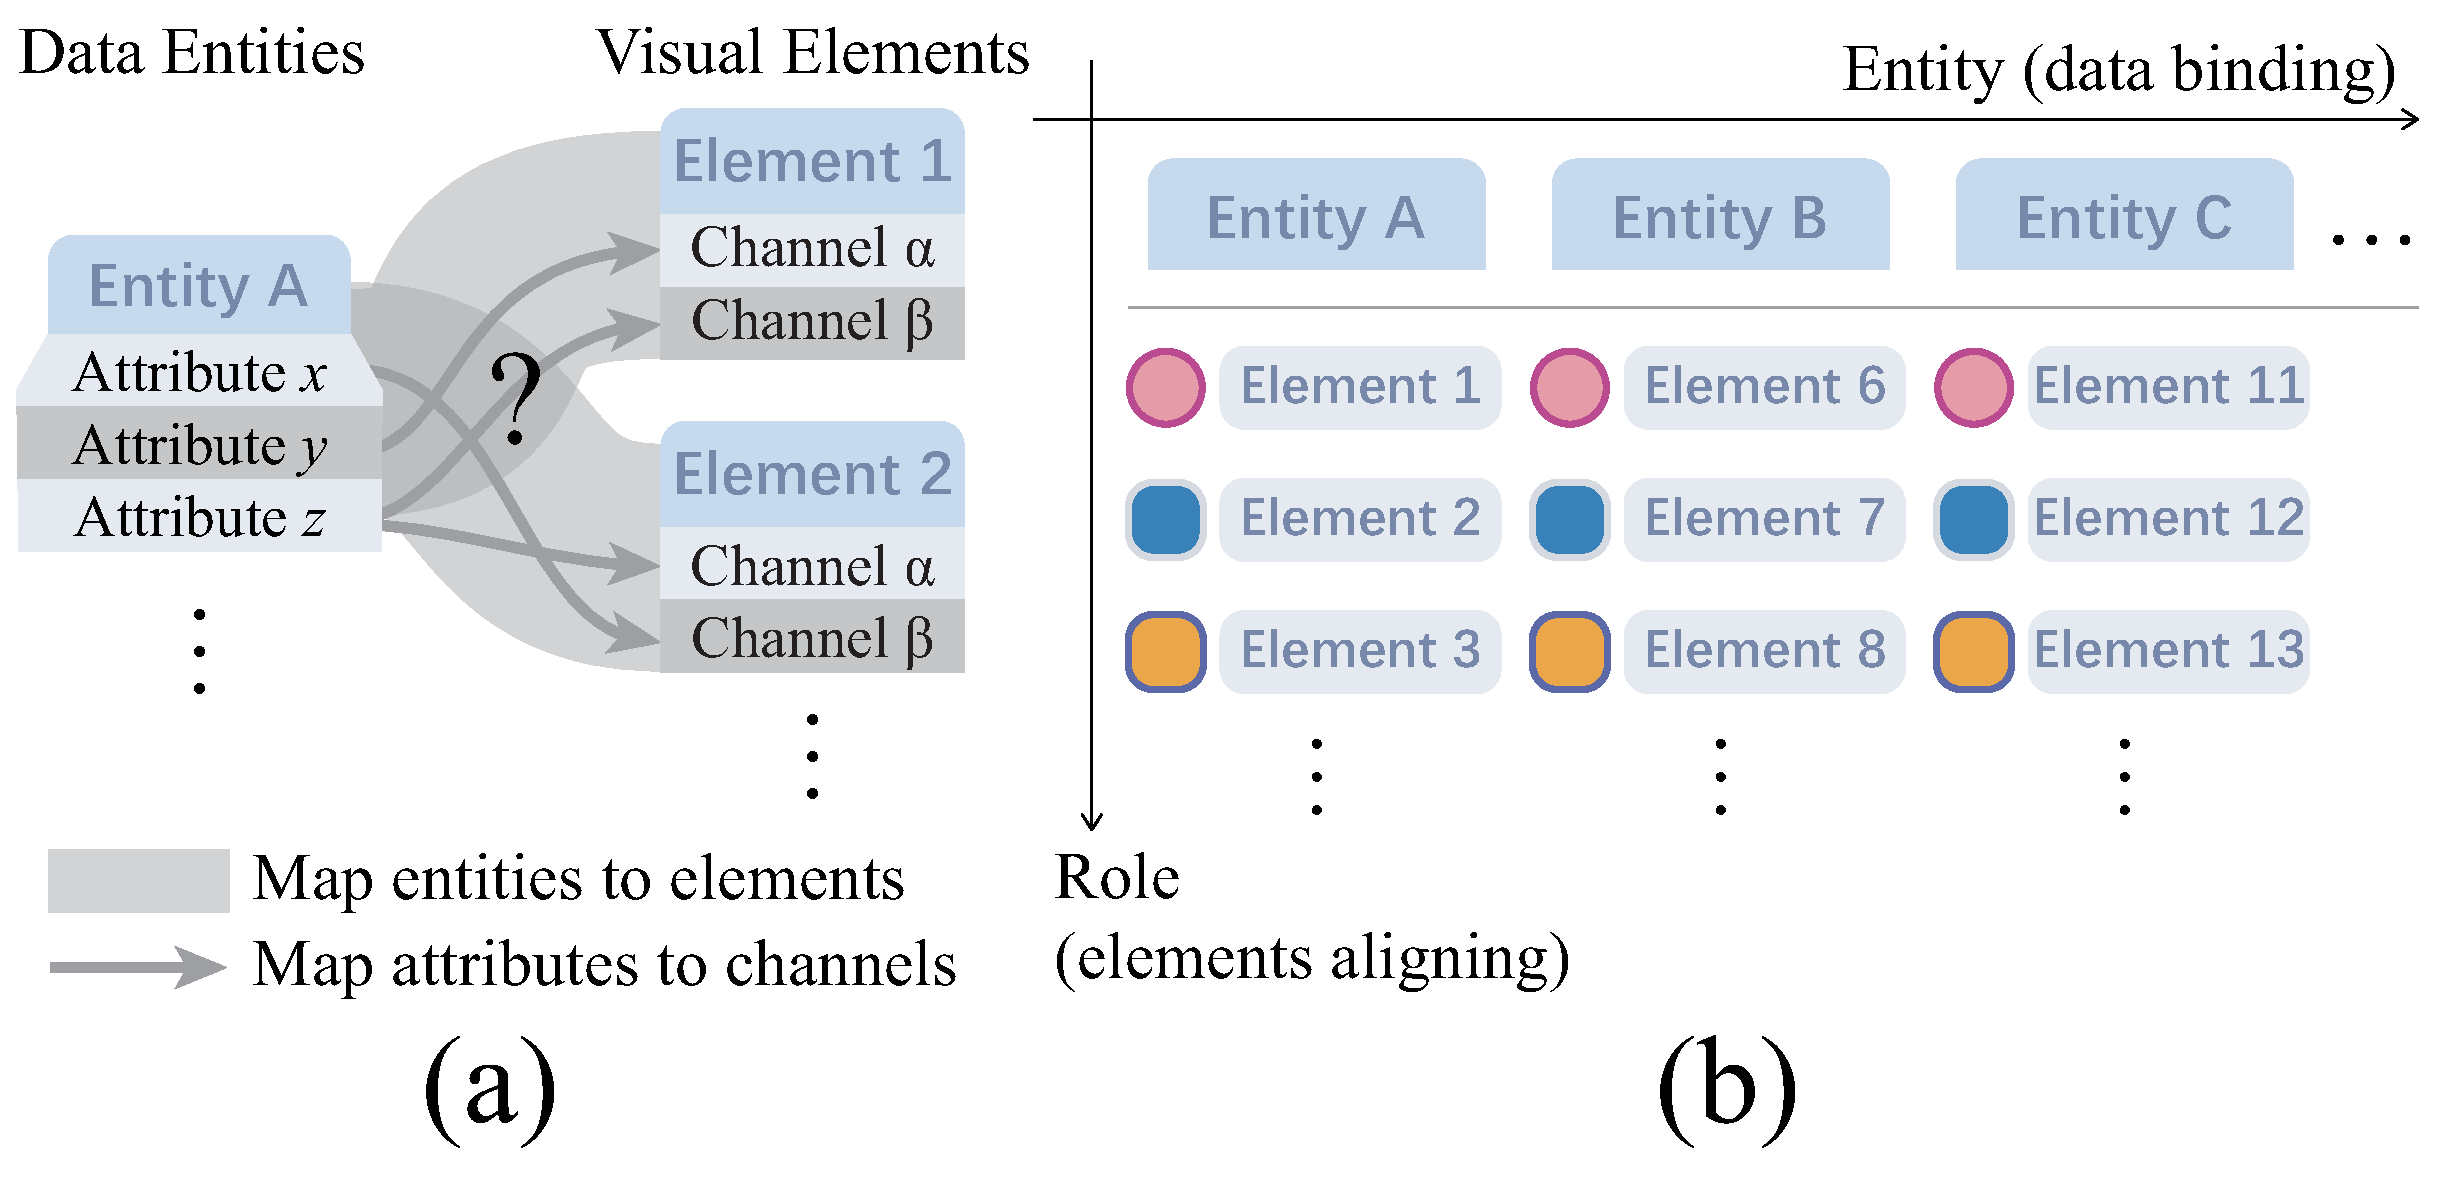
\includegraphics[width=1\columnwidth]{figures/ElementAligning.eps}
    \caption{(a) The target of our visual encoding detection technique; and (b) effect of the data-binding step and the elements-aligning step.}
    \label{fig:ElementAligning}
\end{figure}

% xxxx 等人的工作为我们提供了一个良好的思路,但他们的工作存在一些限制
A tool proposed by Harper and Agrawala~\cite{DBLP:conf/uist/HarperA14} provides a creative perspective for visual encoding extraction.
Although that tool can be extended to support simple node-link diagrams (where each data entity is encoded as only one element), several limitations exist:
\begin{compactenum}
% 1. 其需要创作者使用d3的数据绑定,才能发挥__data__的作用;使用其他工具,或者未将数据绑定到元素上时则无法使用该方法;
\item The D3's data-binding feature is required within the tool so by the ``\texttt{\_\_data\_\_}'' attribute of visual elements can be acquired. 
It cannot deal with general SVG-format visualizations without data bound to visual elements.

% 2. 其只能检验属性和视觉通道之间是否存在线性映射或者类别性映射。
\item It only supports the linear mapping and the categorical mapping and cannot maintain situations with complex visual mappings.
\end{compactenum}
These obstacles prevent it from extracting visual encodings from node-link diagrams created in the general SVG format.

% 我们针对节点链接图的场景,提出了一个数据绑定的策略,通过不断调整输入的数据,检查输出的变化,从而获取数据到svg元素之间的映射关系以及属性到视觉通道之间的映射方式,以解决以上两个问题。
For node-link diagrams, we introduce a new technique to solve such limitations.
Our technique incorporates the source code and the underlying graph data.
The key idea is regarding the source code as a black box.
Our technique modifies the input graph data and detects changes in the output SVG to obtain mappings between data entities and visual elements.
It overcomes the limitations by three steps (Figure~\ref{fig:VisualEncodings}):
(1) \textbf{Data binding} binds elements to different data entities.
(2) \textbf{Elements aligning} aligns elements according to their \textit{roles}. 
(3) \textbf{Encoding mapping} detects correlations among attributes, elements, and visual channels.

\subsubsection{Data Binding} \label{sec:databinding}
To detect mappings between \textbf{\textit{data entities}} and \textbf{\textit{visual elements}}, 
we modify attribute values of data entities and record corresponding visual element changes so as to construct mappings between the modified entity and the changed elements.
However, directly modifying attributes may deform the attribute distribution, and this can influence visual mappings so that elements related to other data entities may also be changed.
% 节点的size属性线性映射到编码该节点的圆形的半径r上,r[i] = (size[i] - min(size)) / (max(size) - min(size)) * max_radius
For example, the node's \texttt{size} attribute is linearly mapped into the radius of the \texttt{<circle>} element encoding the node: 
% $$radius_i = \frac{size_i - min(size)}{max(size) - min(size)} * radius_{max}$$
$radius_i = (size_i - min(size)) / (max(size) - min(size)) * radius_{max}$.
Modifying $size_i$ may broaden the attribute range and changes the linear mapping defined by the attribute range.
We prevent this by merely swapping attributes of two entities rather than modifying them, so that no new data is introduced and the distribution is preserved.
We take nodes as an example.
After swapping all two nodes' attributes, visual elements that differ from the previous are regarded as two nodes' corresponding elements.
For example, after swapping nodes B and C in Figure~\ref{fig:DataBinding} (b), elements 1 to 4 are changed.
All these changed elements correspond to nodes B and C because only B and C are swapped.
After swapping the node B with the node A in Figure~\ref{fig:DataBinding} (c), elements 2 and 3 are changed twice (Figure~\ref{fig:DataBinding} (b) and (c)), thus they correspond to node B because only node B are swapped twice.
% To ensure all elements of node B are detected, we swap it with all the other nodes.
Each node will be swapped with all other nodes to ensure that all elements belonging to it are detected.
After swapping all nodes, the entire node-to-element mapping is constructed (Figure~\ref{fig:DataBinding} (d)).
Node entities are bound to their corresponding elements.
The link-to-element mapping is constructed in the same way.
Because swapping two nodes may influence their related links, node-related elements can contain elements corresponding to links.
We remove elements corresponding to links from the node-to-element mappings.
Two parts ($entity$ and $element$) of the mapping relationship are solved.

\begin{figure}
    \centering
    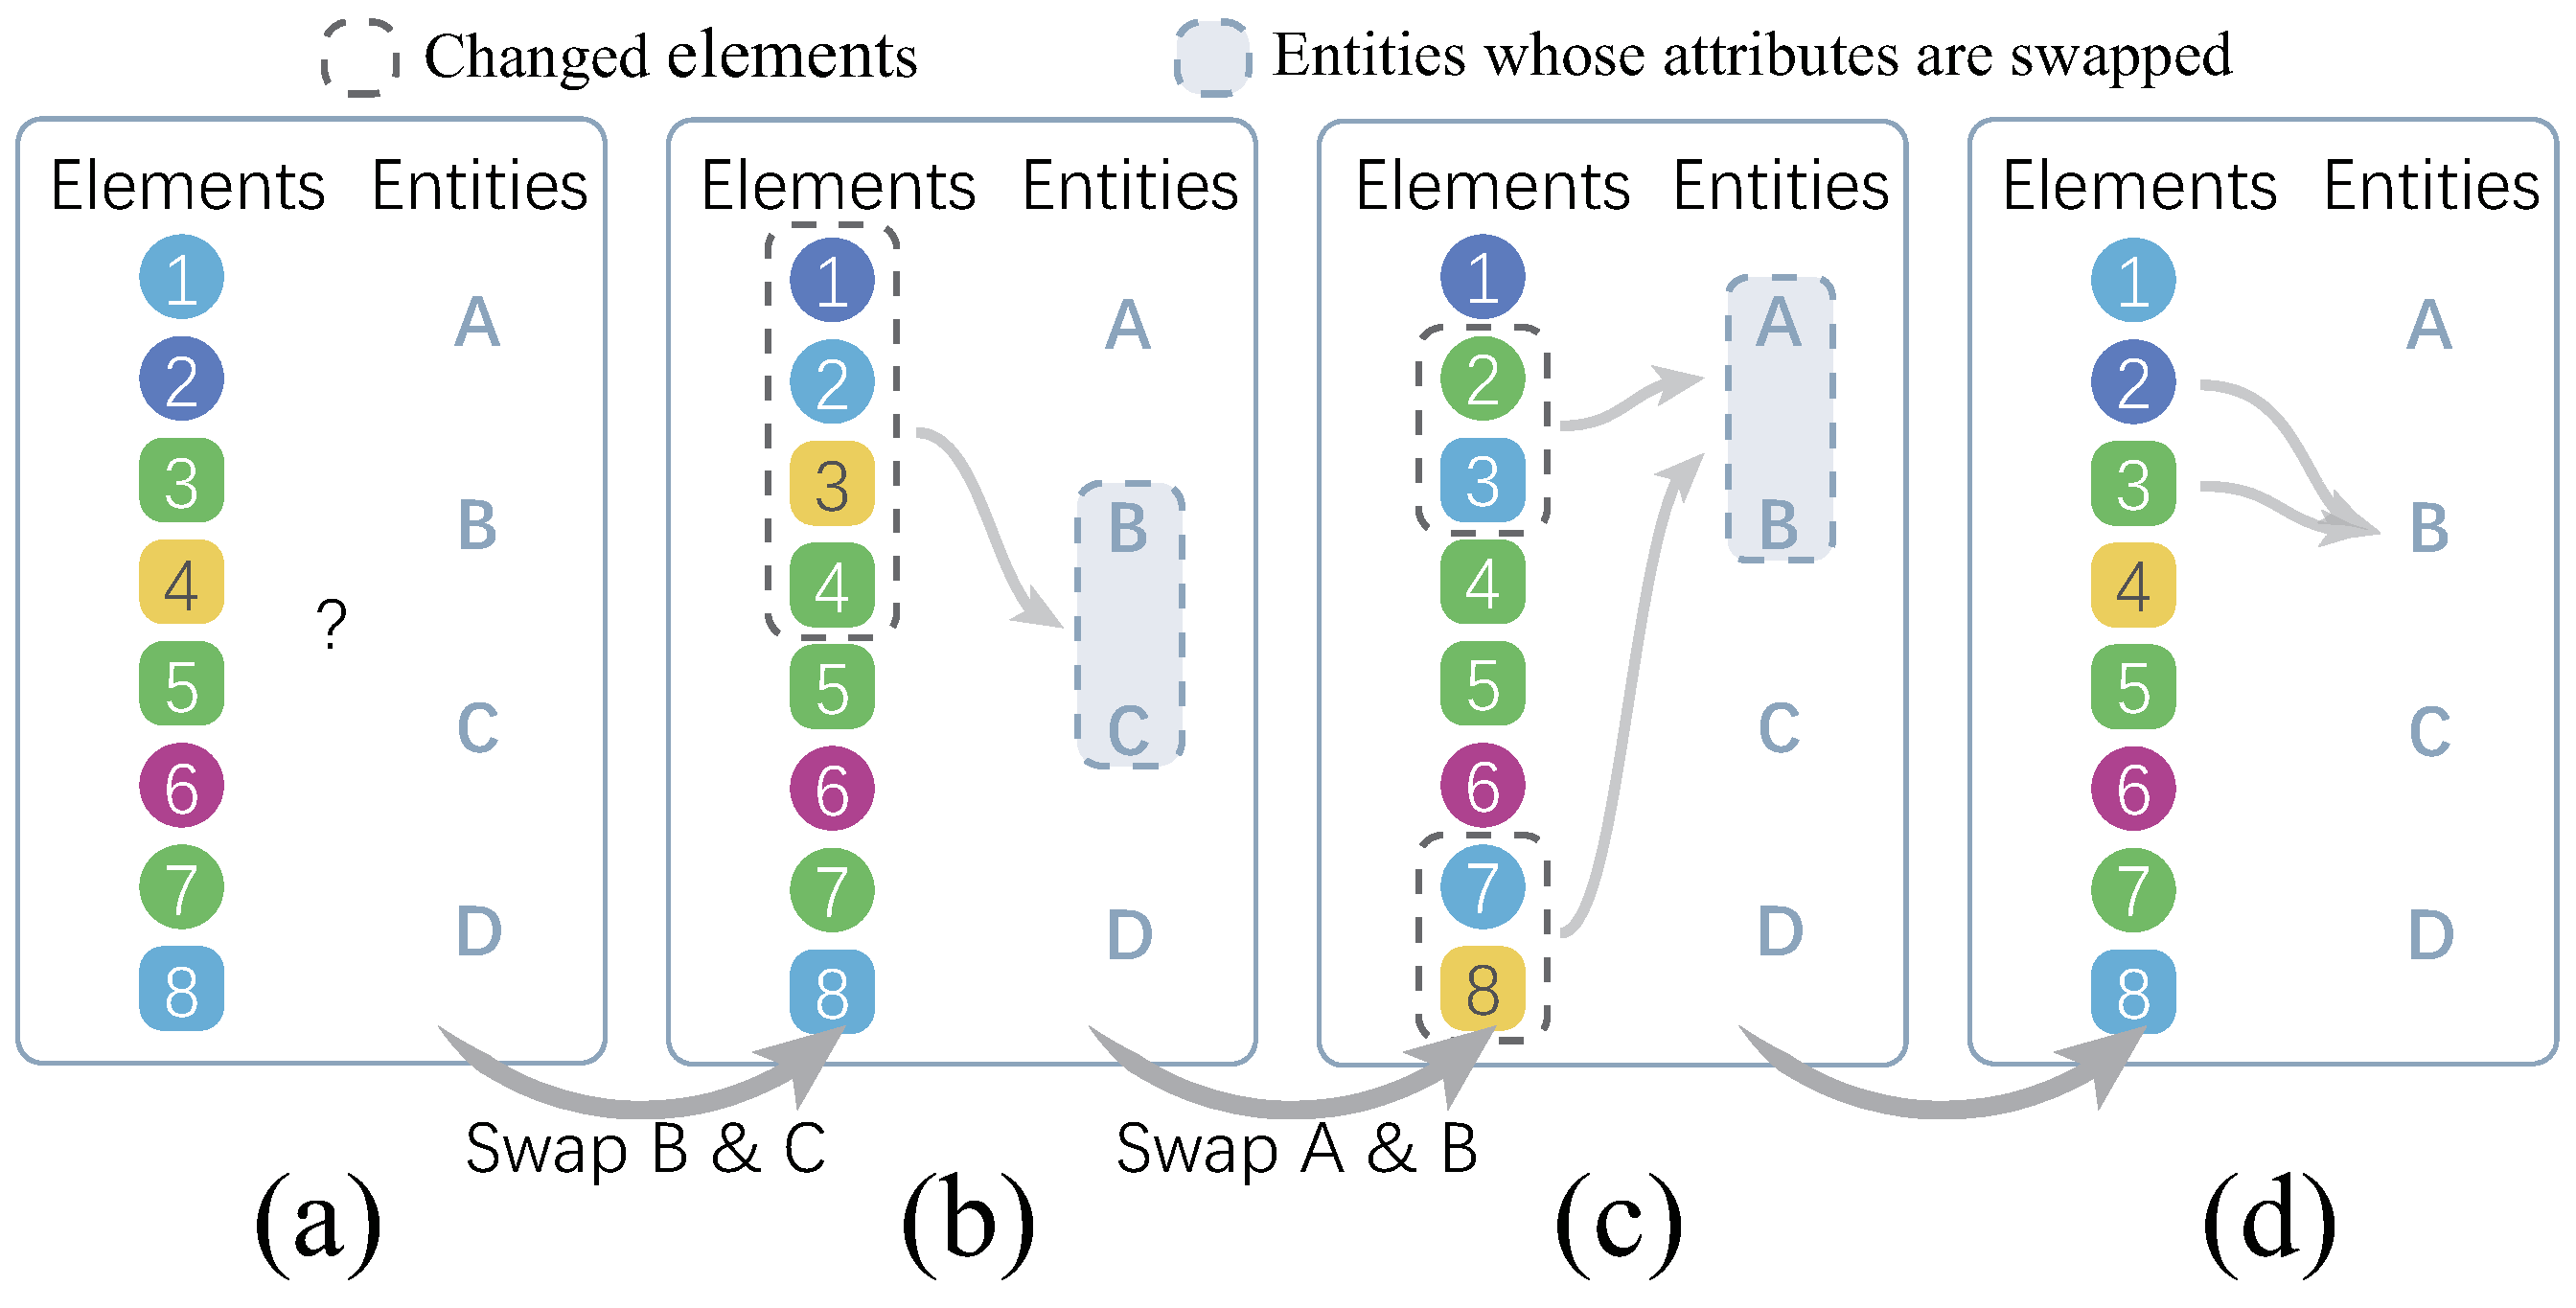
\includegraphics[width=1\columnwidth]{figures/DataBinding.eps}
    \caption{Data binding is achieved by swapping attributes of data entities. (a) Visual mappings between original visual elements and data entities are unknown. (b) After swapping attributes of entities B and C, the appearance of elements 1 to 4 is changed. Thus, entities B and C correspond to elements 1 to 4. (c) After swapping attributes of entities A and B, the appearance of elements 2, 3, 7, and 8 is changed. Thus, entities A and B correspond to these elements. (d) After swapping B with A and C, elements 2 and 3 change twice. We can map entity B to elements 2 and 3.}
    \label{fig:DataBinding}
\end{figure}

\subsubsection{Elements Aligning}
The data-binding step only binds visual elements into different data entities (the horizontal direction in Figure~\ref{fig:ElementAligning} (b)).
The roles of different elements are unknown.
The \textit{role} of an element is defined as a function that maps attributes to visual channels:
\begin{equation}
    role :=  \{attribute: value\} \mapsto \{channel: appearance\}
\end{equation}
% 两个元素相同角色,当且仅当,在它们所对应的数据实体的所有属性都相同时,它们的channels也都一样。
Two elements have the same role iff given arbitrary same inputs (all attributes of their corresponding entities), their outputs (all their visual channels) are the same.
For the example in Figure~\ref{fig:VisualEncodings}, 
roles of all three left inner rectangles are the same,
because if we swap all attributes of nodes A and B, node A's left rectangle before swapping will be same to node B's left rectangle after swapping regarding all their visual channels such as \texttt{x}, \texttt{y}, \texttt{fill}, and \texttt{height}.
They are aligned to classify their roles (the vertical direction in Figure~\ref{fig:ElementAligning} (b)).
% The \textit{role} can be regarded as a function that takes data attributes as input and assign values for visual element channels.
% Elements across different data entities are regarded as the same role if their effects are the same.
% Elements within the same role should appear exactly the same when their own nodes have exactly same attributes.
% 通过测试两个元素在同一属性输入时是否表现一致,来判断它们是否属于一种角色。
Different elements' role identity can be determined by swapping their corresponding data entities along with the data binding step, because all attributes of one entity before swapping are the same to the counterpart of the other one after swapping.
For example, in Figure~\ref{fig:DataBinding} (b), after swapping entity B with entity C, element 1 appear same to element 2 before swapping in Figure~\ref{fig:DataBinding} (a). Thus, elements 1 and 2 can be aligned into the same role.
We clarify the binding among visual elements, data attributes, and visual channels, which is conducive to the subsequent steps.
% 这样做的意义:能够使得数据和可视化之间的绑定更加清晰,有利于后续步骤的进行。


\subsubsection{Encoding mapping}\label{sec:encodingmapping}
The previous two steps classify elements according to two dimensions (the entity and the role) to solve \textbf{Q\ref{qstn:composition}}.
% 到此为止,我们已经已经知道每个实体是由哪些不同角色的元素组成,足够回答第一个问题
However, correlations between visual channels and data attributes are not determined.
% 我们继续以节点为例。
We continue to take nodes as an example.
% 为了检验一个属性究竟被编码在了哪些视觉通道上,我们通过shuffle所有节点的某个属性,观察视觉通道发生的变化。
We detect related visual channels of an attribute by shuffling all nodes' attributes and observing visual channel changes of their corresponding elements.
% 变化可以被定义为,某个属性引起某些元素的某些视觉通道的变化。
One correlation is defined as ``which \textit{attribute} changes which \textit{visual channel} of which \textit{element}''. We formalize it as:
\begin{equation}
    correlation := ( attribute, element, channel )
\end{equation}
% 然后我们根据不同的element角色,对这些发生的变化进行合并。
We merge different correlations according to the role of elements.
Thus, we replace the $element$ in the correlation's definition with $role$.
We obtain the entire correlation set of different roles to solve \textbf{Q\ref{qstn:encodings}}.
% It generates more comprehensive mappings between attributes and visual channels for elements of different roles.

Moreover, we identify the category of correlations to solve \textbf{Q\ref{qstn:correlation}}.
It requires the classification of attribute types and channel types.
We support numerical attributes and categorical attributes in \ApproachName.
List attributes and dictionary attributes are separated into multiple numerical attributes or categorical attributes (e.g.,\texttt{[1, 2, 3]}, \texttt{\{"year":2021,"month":03\}}).
We regard all visual channels as numerical (colors can be divided into RGB channels which are numerical).
However, numerical data can be used as categorical data if there are only a few classes of values.
For example, natural numbers are often used as categorical attributes such as labels, groups, and classes.
Thus, for numerical data, we must compare the number of unique values and their entries to determine whether it is numerical or categorical.
We set up a parameter $\alpha$ to make the distinction: if all values of the attribute are natural numbers and
the number of an attribute's unique values is less than $\alpha$ percent of the number of data entities, we regard the attribute as categorical.
% 我们根据属性和通道的类型来定义关系的类型
We identify the type of correlation by the type of attribute and channel:
\begin{compactitem}
    \item \textbf{The channel and attribute are categorical} or \textbf{the channel is categorical while the attribute is numerical}. 
    % 为了描述不同的channel取值所代表的的含义。我们为每类不同的channel记录了它们所对应的属性的取值范围。
    In order to describe the meanings of different channel values,
    We record the value range of the attribute for each category of channel values.
    % 假如在这种关系下,不同类别的channel对应的属性取值有交叉,我们则会抛弃这种关系,因为它具有歧义。
    If the attribute values corresponding to different channel values intersect, we discard this correlation because it is ambiguous.
    
    \item \textbf{The channel and attribute are numerical}. We compute the Pearson's Correlation Coefficient and test whether the correlation is positive, negative, or uncorrelated with the coefficient and the significance test's p-value. We take the attribute as a factor that influences the visual channel when the absolute value of the coefficient is larger than $\theta$, and the $p$-value of the significance test is less than $\alpha$. We set $\theta = 0.5$ and $\alpha = 0.05$ by default, both parameters can be adjusted on-demand.
\end{compactitem}
The correlation type where \textbf{the channel is numerical while the attribute is categorical} is not supported because it is counterintuitive.


\begin{algorithm}[!t]
    \renewcommand\arraystretch{1.2}
    \caption{ Visual Encodings Textualization }
    \label{alg:textualize}
    \begin{algorithmic}[1]
        % \Require
            % $G=(V=\{v_1, v_2, ..., v_n\}, E=\{e_1, e_2, ..., e_n\})$: a graph;
        % \Ensure
            % $C$: the potential condition set
        % \State Init conditions $C=\varnothing$, false conditions $FC=\varnothing$
        \State // Describing Nodes
        \State Describing \textbf{Q\ref{qstn:composition}}: what \textit{elements} (\textit{roles}) does a node consist of? \label{alg:VsEnNodeConsist}
        \For {each \textit{role} in a node} \label{alg:VsEnEachRole}
            \If {its \texttt{tagName} does not encode any \textit{attribute}}
                \For {each \textit{visual channel} that encodes some attributes}
                    \State Describing \textbf{Q\ref{qstn:encodings}}: how \textit{channel} encodes \textit{attributes}? \label{alg:VsEnQ2-1}
                    \State Describing \textbf{Q\ref{qstn:correlation}}: the type of their \textit{correlations}
                    \label{alg:VsEnQ3-1}
                \EndFor
            \EndIf
            \If {its shape (\texttt{tagName}) encodes some attributes}
                \For {each \textit{visual channel} that all shapes share}
                    \State // e.g., \texttt{fill} and \texttt{stroke-width}
                    \State Describing \textbf{Q\ref{qstn:encodings}}: how \textit{channel} encodes \textit{attributes}? \label{alg:VsEnQ2-2}
                    \State Describing \textbf{Q\ref{qstn:correlation}}: the type of their \textit{correlations}
                    \label{alg:VsEnQ3-2}
                \EndFor
                \State Describing all its shapes \label{alg:VsEnTagName}
                \For {each shape (\texttt{tagName})}
                    \State Describing \textbf{Q\ref{qstn:encodings}}: how \textit{channel} encodes \texttt{tagName}? \label{alg:VsEnQ2-3}
                    \State Describing \textbf{Q\ref{qstn:correlation}}: the type of their \textit{correlations}
                    \label{alg:VsEnQ3-3}
                    \For {each \textit{visual channel} that this shape holds}
                        \State // e.g., \texttt{rx} and \texttt{ry}
                        \State Describing \textbf{Q\ref{qstn:encodings}}: how \textit{channel} encodes \textit{attributes}? \label{alg:VsEnQ2-4}
                        \State Describing \textbf{Q\ref{qstn:correlation}}: the type of their \textit{correlations} \label{alg:VsEnQ3-4}
                    \EndFor
                \EndFor
            \EndIf
        \EndFor
        \State // Describing Links ...
    \end{algorithmic}
\end{algorithm}

\subsubsection {Template-based Textualization}
Descriptions of visual encodings are generated based on several templates.
There are logical and hierarchical relationships in the narration of these visual encodings.
Algorithm~\ref{alg:textualize} summarizes the overall logic for describing visual encodings.
We describe nodes and links respectively.
Elements of different roles composing a node are narrated separately, for example,
\textit{``Each @node consists of @4 different elements.''} (line~\ref{alg:VsEnNodeConsist}),
\textit{``The @first element is a @\texttt{<rect>}.''} (line~\ref{alg:VsEnEachRole}).
% 为了标记模板中用于填充信息的部分,我们对这些位置进行了高亮。
To mark the placeholders of templates that are used to fill in the information, we place a @ sign before the words that fill into these placeholders.
For visual channels that encode attributes, we describe their correlation to solve \textbf{Q\ref{qstn:encodings}} and \textbf{Q\ref{qstn:correlation}}.
For example, \textit{``Its @fill encodes the attribute @group.''} (line~\ref{alg:VsEnQ2-1}).
% , \textit{``The greater the attribute @value is, the @greater its @stroke-width is.''} (line~\ref{alg:VsEnQ3-1},~\ref{alg:VsEnQ3-2},~\ref{alg:VsEnQ3-3}, and~\ref{alg:VsEnQ3-4}).
If the correlation is categorical-to-categorical, we describe different categories separately: \textit{``When the value of @group is @2, its @fill is changed into @darkorange (\#ff7f0e).''} (Colors are described as the most similar color in a predefined set of colors with 146 different names).
If the correlation is numerical-to-numerical, we describe whether the value of the channel will increase or decrease with the growth of the attribute's value: \textit{``The greater the attribute @value is, the @greater its @stroke-width is.''} (line~\ref{alg:VsEnQ3-1}).

If the shape is used to encode some attributes, the logic of description is different.
We first describe common channels shared by different shapes (lines~\ref{alg:VsEnQ2-2} and~\ref{alg:VsEnQ3-2}) and then narrate different shapes:
\textit{``Its tagName varies from @\texttt{<circle>} and @\texttt{<rect>}.''} (line~\ref{alg:VsEnTagName}), \textit{``When the value of @country is @France, its tagName is changed into @\texttt{<circle>}``} (lines~\ref{alg:VsEnQ2-3} and~\ref{alg:VsEnQ3-3}), and \textit{``Its @radius encodes the attribute @votes. The greater the @votes, the @greater its @radius.''}(lines~\ref{alg:VsEnQ2-4} and~\ref{alg:VsEnQ3-4}).

\subsection{Interpreting Layout Intention}
% Layouts of attributed graphs have been categorized into attribute-based layouts~\cite{} and topology-based layouts~\cite{} by Nobre et al.~\cite{DBLP:journals/cgf/NobreMSL19}.
Nobre et al.~\cite{DBLP:journals/cgf/NobreMSL19} categorized layouts of attributed graphs into attribute-based layouts~\cite{DBLP:journals/tvcg/ElzenW14, DBLP:journals/tvcg/Guo09} and topology-based layouts~\cite{DBLP:journals/spe/FruchtermanR91, DBLP:journals/cgf/KruigerRMKKT17, DBLP:journals/tvcg/GansnerHN13, DBLP:journals/tvcg/ZhuCHHLZ21}.
The core of describing layout intention is to determine whether the layout is attribute-based or topology-based, is handled in two steps: 

\textbf{1) Capturing the position of each node}.
To capture each node's position, we compute a bounding box for elements detected in Section~\ref{sec:databinding}.
The bounding box of a node is the smallest rectangle that contains all its corresponding elements.
We take the centroid of the bounding box as the position of the node.

\textbf{2) Determining the layout type.} 
The attribute-based category of layouts is defined as algorithms that mapping node attributes to the two dimensions ($x$ and $y$) of the Cartesian coordinate. 
We utilize the Pearson correlation test same to Section~\ref{sec:encodingmapping} to test whether an attribute relates to the layout.
% For each attribute of the node, we test whether it relates to the layout.
% The test is similar to the correlation test in Section~\ref{sec:encodingmapping}.
% If the test does not suggest any attribute as the impact factor, we begin to test whether it is topology-based.
For topology-based layouts, we assume that their graph geodesic distance influences the Euclidean distance between two nodes.
The Pearson correlation coefficient can also be used to test the correlation.
We assume that with the conditions that the Pearson correlation coefficient is more significant than $\theta$ and $p$-value is smaller to $\alpha$, the layout is topology-based.

Thus we first perform a pre-study to validate our hypothesis.
% 找N个不同的数据集(跨不同领域),找几种不同种类的拓扑based的layout;检验他们的pearson值,p值等等;比较它们在随机布局下的结果;
We prepare 15 different graph datasets from~\cite{DBLP:journals/tvcg/ZhuCHHLZ21}.
The number of their nodes varies from 72 to 1083, and the number of their links varies from 75 to 8677.
They are collected from diverse areas such as literature, music, research, and social media.
We layout them using five different kinds of topology-based layouts with default parameters: FM$^3$~\cite{hachul2004drawing}, Fruchterman-Reingold spring layout (F.R.)~\cite{DBLP:journals/spe/FruchtermanR91}, Stress Majorization (S.M.)~\cite{DBLP:conf/gd/GansnerKN04}, Pivot MDS (PMDS)~\cite{DBLP:conf/gd/BrandesP06}, and Radial Tree layout (R.T.)~\cite{DBLP:conf/infovis/Jankun-KellyM03}.
% 我们还检验了随机布局是否也符合我们的假设
We also test whether the random layout conforms to our assumption.
We highlight cells where the Pearson correlation coefficient is smaller than $\theta$ in Table~\ref{tab:pearson-correlation}.
They suggest that correlations between the euclidean distance and the graph geodesic distance are weak.
$p$-values are all zero for the five topology-based layouts in all 15 datasets.
They suggest strong correlations between the Euclidean distance and the graph geodesic distance.
However, nine of 15 datasets with the random layout also produce $p$-values less than $\alpha$, which suggests they are significant.

% 这些基于拓扑的布局产生的节点位置,能够使节点间的欧式距离反应它们的拓扑距离。
Two tables indicate that in most cases, the Euclidean distance between two nodes reflects their graph geodesic distance with topology-based layouts.
% 在大部分情况下,使用pearson 相关系数>0.6且p-value<0.05来检验是否该布局为拓扑布局是可行的。
Thus, it is feasible to study whether the layout is a topological layout with the first condition established (the Pearson correlation coefficient$>\theta$).

Descriptions of the layout intention are also template-based.
For attribute-based layout, we narrate that: \textit{``The @x-coordinate encodes the attributes @votes''}.
The description for topology-based layouts is: \textit{``The layout is a topology-based layout, which means the farther the topology distance between two nodes, the farther the distance between them''}.
When the layout does not conform to the two categories, it yields: \textit{``The layout is neither an attribute-based layout nor a topology-based layout.''}.

\begin{table}[ht]
\caption{\label{tab:pearson-correlation}The Pearson correlation coefficients testing correlations between Euclidean distances and graph geodesic distance with 15 graphs and 6 different layouts. Cells with coefficients less than $\theta=0.5$ are highlighted.}

\setlength{\tabcolsep}{1.5mm}{

% \resizebox{\textwidth}{15mm}{
\begin{tabular}{lllllll}
\hline
Dataset       & FM$^3$ & F.R.           & S.M.  & PMDS  & R.T.           & Random          \\ \hline
dwt\_72       & 0.894                 & 0.552          & 0.94  & 0.897 & 0.714          & \textbf{-0.003} \\
lesmis        & 0.804                 & 0.728          & 0.815 & 0.779 & 0.504 & \textbf{-0.03}  \\
bcsstk09      & 0.967                 & 0.610          & 0.971 & 0.947 & 0.754          & \textbf{-0.008} \\
cage8         & 0.658                 & 0.678          & 0.725 & 0.701 & \textbf{0.307} & \textbf{-0.002} \\
can\_96       & 0.835                 & 0.824          & 0.855 & 0.869 & \textbf{0.426} & \textbf{0.013}  \\
dwt\_1005     & 0.969                 & 0.561          & 0.974 & 0.972 & 0.623          & \textbf{0.007}  \\
dwt\_419      & 0.979                 & \textbf{0.391} & 0.987 & 0.987 & 0.775          & \textbf{-0.004} \\
grid17        & 0.968                 & 0.551          & 0.976 & 0.964 & 0.738          & \textbf{-0.007} \\
jazz          & 0.826                 & 0.821          & 0.813 & 0.786 & \textbf{0.297} & \textbf{0.004}  \\
mesh3e1       & 0.99                  & 0.502          & 0.996 & 0.995 & \textbf{0.465} & \textbf{0.002}  \\
netscience    & 0.901                 & 0.573          & 0.93  & 0.919 & 0.752          & \textbf{-0.018} \\
price\_1000   & 0.783                 & \textbf{0.376} & 0.808 & 0.786 & 0.727          & \textbf{-0.007} \\
rajat11       & 0.753                 & 0.670          & 0.868 & 0.847 & 0.618          & \textbf{-0.064} \\
soc-wiki-Vote & 0.798                 & 0.775          & 0.821 & 0.757 & \textbf{0.316} & \textbf{-0.01}  \\
visbrazil     & 0.937                 & 0.828          & 0.941 & 0.958 & 0.758          & \textbf{0.01}   \\ \hline
\end{tabular}}
\end{table}

% \begin{table}[ht]
% \caption{\label{tab:pearson-pvalue}Pearson p-value(TODO).}

% \setlength{\tabcolsep}{1.9mm}{

% \begin{tabular}{lllllll}
% \hline
% Dataset       & FM$^3$ & F.R. & S.M. & PMDS & R.T. & Random         \\ \hline
% dwt\_72       & 0                     & 0    & 0    & 0    & 0    & \textbf{0.842} \\
% lesmis        & 0                     & 0    & 0    & 0    & 0    & 0.021          \\
% bcsstk09      & 0                     & 0    & 0    & 0    & 0    & 0              \\
% cage8         & 0                     & 0    & 0    & 0    & 0    & 0.027          \\
% can\_96       & 0                     & 0    & 0    & 0    & 0    & \textbf{0.203} \\
% dwt\_1005     & 0                     & 0    & 0    & 0    & 0    & 0              \\
% dwt\_419      & 0                     & 0    & 0    & 0    & 0    & \textbf{0.111} \\
% grid17        & 0                     & 0    & 0    & 0    & 0    & \textbf{0.060} \\
% jazz          & 0                     & 0    & 0    & 0    & 0    & \textbf{0.421} \\
% mesh3e1       & 0                     & 0    & 0    & 0    & 0    & \textbf{0.604} \\
% netscience    & 0                     & 0    & 0    & 0    & 0    & 0              \\
% price\_1000   & 0                     & 0    & 0    & 0    & 0    & 0              \\
% rajat11       & 0                     & 0    & 0    & 0    & 0    & 0              \\
% soc-wiki-Vote & 0                     & 0    & 0    & 0    & 0    & 0              \\
% visbrazil     & 0                     & 0    & 0    & 0    & 0    & 0.025          \\ \hline
% \end{tabular}}

% \end{table}

\subsection{Interactive Descriptions}
Descriptions can be enhanced by interactions because they are generated with corresponding elements.
For example, descriptions about nodes correspond to nodes related elements.
When audiences hover on one sentence of description, we highlight related elements to help the user capture the description's target.
We develop an interactive web-based interface by JavaScript to support generating interactive descriptions (Figure~\ref{fig:interface}) with \ApproachName.
Creators can write visualization code in the Code Editor and input the graph data in the Data Editor.
\ApproachName~generates the visualization results and their corresponding interactive descriptions.


\begin{figure}[ht]
    \centering
    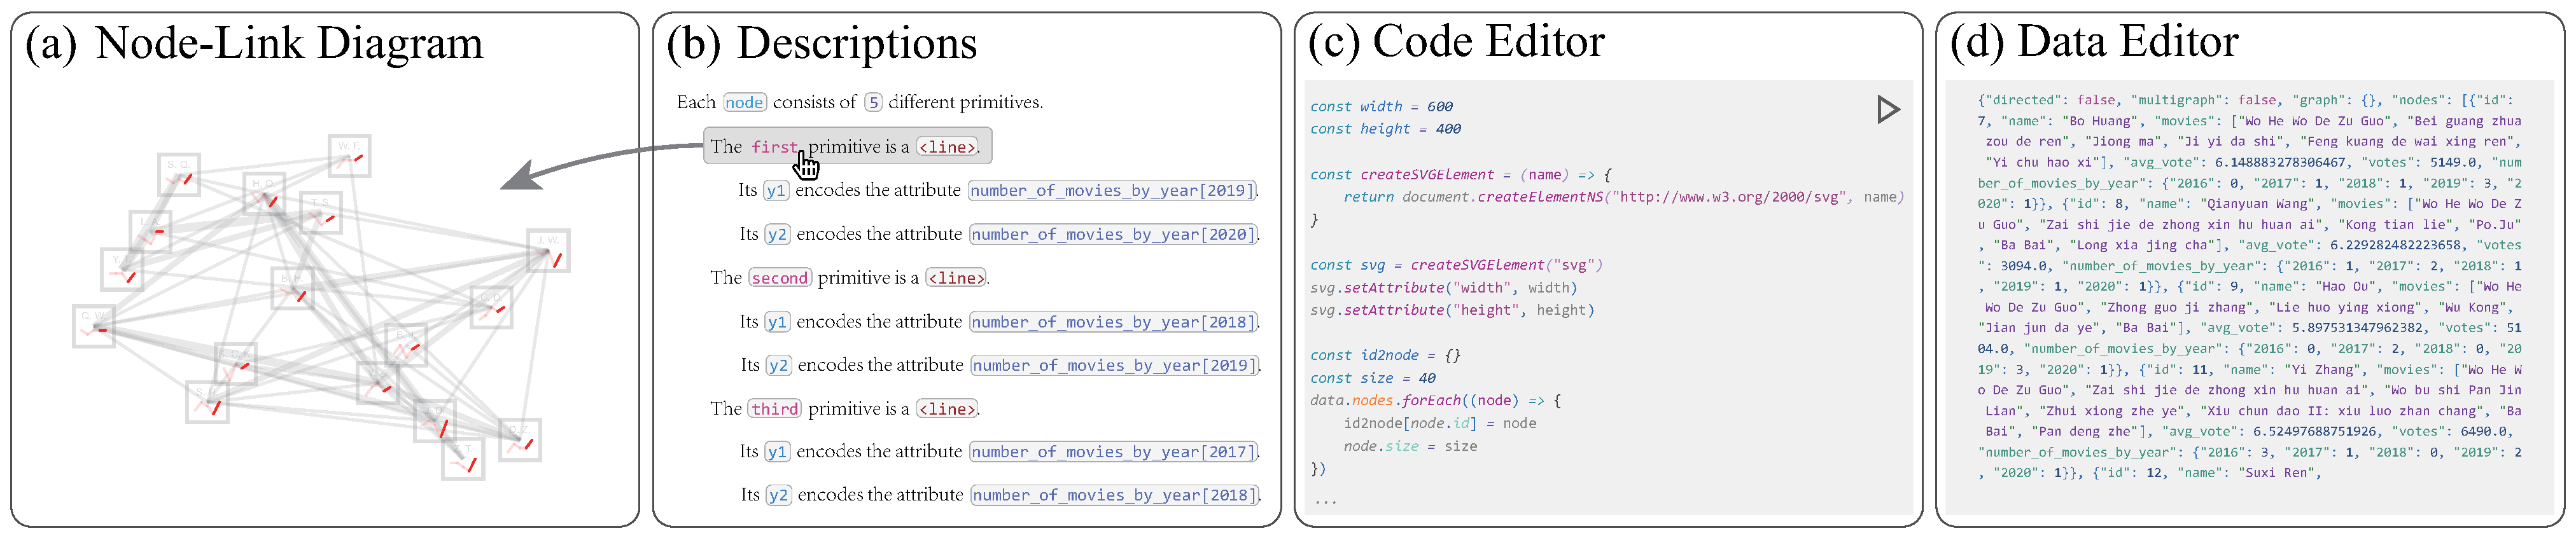
\includegraphics[width=1\columnwidth]{figures/interface.eps}
    \caption{The interface consists of four parts: (a) the node-link diagram view, (b) the descriptions view that shows the descriptions generated by \ApproachName, (c) the code editor view where creators can edit their visualization creation code, and (d) the data editor where creators input the graph data.}
    \label{fig:interface}
\end{figure}
\fi
%********************* ************************* *********************%
\section{Case Studies}
We conduct four case studies to demonstrate descriptions generated by \ApproachName.
The IMDb movie dataset~\footnote{\url{https://www.imdb.com/}} has been used in plenty of works~\cite{DBLP:journals/tvcg/SrinivasanPEB18, DBLP:journals/pvldb/KrishnanWWFG16, DBLP:conf/ieeevast/BigelowNML19}.
We employ it to conduct our case studies.


\subsection{Case 1: Simple Nodes and Links}\label{sec:imdb_movies}
The result of Case 1 is available in Figure~\ref{fig:BasicCases} (a) and (c).
This case is aimed to show a basic example.
% 我们挑选了数据集中2019年在中国上映的电影。
\textbf{1) Graph Wrangling}. We select movies in the dataset which is published in 2019 and is released in China.
% 我们保留了其中标题、发布日期、演员、类别、
We preserve seven attributes for movies: \texttt{"title"}, the publish date (\texttt{"date\_published"}), \texttt{"actors"}, \texttt{"genre"}, \texttt{"director"}, \texttt{"writer"}, and \texttt{"country"}.
Two movies are connected if they share at least one same actor.
We generate an attribute, \texttt{"shared\_actors"}, for each link. 
It records the number of shared actors.
We totally obtain 49 nodes and 99 links.
\textbf{2) Visual Encodings}. 
Nodes are visualized as \texttt{<circle>}s and links are visualized as \texttt{<line>}s (Figure~\ref{fig:NodeLineChartsCase} (a)).
The fill colors of \texttt{<circle>}s encode their publish seasons (e.g., when \texttt{"date\_published"} is \texttt{01}, \texttt{02}, or \texttt{03}, it means the publish season is spring, we fill the node with \texttt{"steelblue"}).
The width of \texttt{<line>}s encode the \texttt{"shared\_actors"}.
\textbf{3) Layout Computing}. 
We pre-compute a layout with a spring layout algorithm~\cite{DBLP:journals/spe/FruchtermanR91}.

\textbf{Results}.
The descriptions are generated for the created node-link diagram (Figure~\ref{fig:NodeLineChartsCase} (e)).
They can be separated into three parts:

\textbf{1) Interpreting Linking Conditions.} Several conditions (e.g. (\texttt{"C2"}, \texttt{"country"}, \texttt{"China"}), (\texttt{"C1"}, \texttt{"year"}, \texttt{"2019"}), etc.) are detected but only the condition (\texttt{"C2"}, \texttt{"actors"}, \texttt{"[arbitrary value]"}) is preserved because other conditions also are held on unconnected node pairs.
Thus \ApproachName~describes the linking condition as \textit{``Two nodes are connected if their attributes {\texttt{actors}} have common values''}.

\textbf{2) Interpreting Visual Encodings.} All visual encodings are detected by \ApproachName~as expected.
Whereas, our technique does not detect that the color of each node encodes the publish season because ``season'' is an abstract concept that are not under our consideration.
However, it generates the mapping of different color categories: 
\textit{``When the value of the attribute {\texttt{date\_published[month]}} is {\texttt{04}}, {\texttt{06}}, or {\texttt{05}}, 
its {\texttt{fill}} turns to {\texttt{darkorange (\#ff7f0e)}}.$\ldots$''}, 
where \texttt{"date\_published[month]"} means the \texttt{"month"} field of the attribute publish date (\texttt{"date\_published"}).
Such descriptions are repeated generated to describe four different \texttt{fill} colors.
Such that audience can obtain that the fill color encodes the ``season''.

\textbf{3) Interpreting Layout Meanings.} \ApproachName~detects the nodes are placed with a topology-based layout. 
Detection of the specific type of the layout is not supported in our technique.
Thus, \ApproachName~only describes the meaning of the topology-based layout in Figure~\ref{fig:NodeLineChartsCase} (e) (Layout Meanings): \textit{``the greater the graph geodesic distance between two nodes is, the greater the euclidean distance between them is''}.

Such descriptions can also facilitate code debugging. 
For example, if the creator negligently encodes the \texttt{fill} color with its publish date,
our technique will detect it and generate descriptions as: \textit{``Its \texttt{fill} encodes the attribute \texttt{date\_published[day]}''}.

\begin{figure*}[ht]
    \centering
    \setlength{\belowcaptionskip}{-5pt}
    \includegraphics[width=2\columnwidth]{figures/NodeLineChartsCase.eps}
    \caption{xxx}
    \label{fig:NodeLineChartsCase}
\end{figure*}

\subsection{Case 2: Nodes with Different Shapes}
Shapes (\texttt{tagName}s) of elements are often used to encode categorical attributes.
This case demonstrates what descriptions will be generated with \ApproachName~where the shape of a node is used to encode a categorical attribute (Figure~\ref{fig:BasicCases.eps} (b) and (d)).

\textbf{1) Graph Wrangling}. 
We select movies directed by Jean-Pierre Melville, a French director. 
Movies are connected if they have common actors. 
We finnally obtain 14 nodes (movies) and 25 links.

\textbf{2) Visual Encodings}.
Movies directed by Melville were most published in France, several of them were published in Italy.
We use square nodes to encode movies published in Italy and circular nodes to encode movies published in France.
The size encodes the number of votes (\texttt{"votes"}) they have received.
The color encodes their main genre (the first genre in their genre attribute \texttt{"genre"}).

\textbf{3) Layout Computing}.
The x and y coordinates encode the publish year (\texttt{"year"}) and the \texttt{"duration"} separately.

\textbf{Results}.
Different from the former case, nodes are visualized with two different elements: \texttt{<circle>} and \texttt{<rect>}.
Their visual channels have differences.
Thus, \ApproachName~describes them separatly:
\textit{``Its \texttt{tagName} encodes the attribute country.
When the \texttt{"country"} is \texttt{France}, its \texttt{tagName} turns to \texttt{<circle>}.
When the \texttt{"country"} is \texttt{Italy}, its \texttt{tagName} turns to \texttt{<rect>}.
When it turns to \texttt{<circle>}, 
its \texttt{r} encodes the attribute \texttt{"votes"}.
When it turns to \texttt{<rect>}, its \texttt{width} and \texttt{height} encode the attribute \texttt{"votes"}.''}.

Another difference is that the layout is attribute-based.
Our technique detects the meanings of two coordinates by testing correlations between node positions and attributes: 
\textit{``The \texttt{x}-coordinate encodes the attributes \texttt{year}. 
The greater the \texttt{year} is, the greater the x-coordinate is.
The \texttt{y}-coordinate encodes the attributes \texttt{duration}.
The greater the \texttt{duration} is, the greater the \texttt{y}-coordinate is.''}.

\subsection{Case 3: Line Charts Embeded on Nodes}
With the IMDb movie dataset, we introduce another case which focuses on actors (Figure~\ref{fig:NodeLineChartsCase} (b) and (f)).
This case focuses on demonstrating more complex situations where each node consists of multiple elements.

\textbf{1) Graph Wrangling}. We first select movies in the dataset that are only released in China from 2016 to 2021.
Their actors who have acted in more than five movies are regarded as nodes.
Each actor has five attributes: \texttt{"name"}, movies s/he acted in from 2016 to 2021 (\texttt{"movies"}), the average vote (\texttt{"avg\_vote"}), the number of votes s/he got (\texttt{"votes"}), the number of movies in each year from 2016 to 2021 (\texttt{"number\_of\_movies\_by\_year"}).
Two actors are connected if they acted in at least one movie from 2016 to 2021.
Finally we obtain 17 nodes and 55 links.

\textbf{2) Visual Encodings}. 
Each node (actor) contains an attribute named \texttt{"number\_of\_movies\_by\_year"}, which has five properties: 2016, 2017, 2018, 2019, and 2020.
Each property stores the number of movies the actor acted in that year.
Following the node-link diagram created by Junker et al.~\cite{DBLP:journals/bmcbi/JunkerKS06}, 
we embed a simple line chart for each node to show the number of movies s/he acted in from 2016 to 2021 (Figure~\ref{fig:NodeLineChartsCase} (a)). 
The width of the link's \texttt{<line>} encodes its attribute \texttt{"number\_of\_shared\_movies"}.

\textbf{3) Layout Computing}. We utilize the layout to show two attributes (\texttt{"avg\_vote"} and \texttt{"votes"}) of each node. The x-coordinate encodes the attribute \texttt{"votes"} and the y-coordinate encodes the \texttt{"avg\_vote"}.

Different with Section~\ref{sec:imdb_movies}, in this case, each node consists of several elements.
We bind elements to different entities and distinguish their roles.
We interpret the meaning of the line chart by describing its elements.
As described in the Visual Encodings part in Figure~\ref{fig:NodeLineChartsCase} (b), it contains five elements.
The first four elements are \texttt{<line>}s.
% 它们组合在一起编码了每个演员每年出演电影数量的趋势,
They are composed together to encode the trend of the actors activeness, namely the number of movies they acted in each year.
Descriptions like \textit{``encode the trend of the actors activeness''} are domain-knowledge based,
% 我们的技术旨在通过生成一些细粒度的描述,帮助观众形成更复杂的认知。
our technique aims to generate fine-grained descriptions to help audiences to form complex cognitions.
% 于是我们的方法对它们的y值分别进行了描述:
It describes them separately: 
\textit{``The first element is a \texttt{<line>}. 
Its \texttt{y1} encodes the attribute \texttt{"number\_of\_movies\_by\_year[2019]"}. 
The greater the \texttt{"number\_of\_movies\_by\_year[2019]"} is, the greater its \texttt{y1} is. 
Its \texttt{y2} encodes the attribute \texttt{"number\_of\_movies\_by\_year[2020]"}.
The greater the \texttt{"number\_of\_movies\_by\_year[2020]"} is, the greater its \texttt{y2} is.''}
Then the description are repeated with different elements and attribtues.
Such descriptions are fine-grained and can be composed to face complex tasks in the future.


\subsection{Case 4: Bars on Links}
Case 4 aims to demonstrate the generated descriptions for links.
The design of the node-link diagram follows Sch{\"{o}}ffel et al.~\cite{DBLP:conf/iv/SchoffelSE16}, links are encoded with several bars to display link attributes.

\begin{figure*}[ht]
    \centering
    \includegraphics[width=2\columnwidth]{figures/LinkBarsCase.eps}
    \caption{xxx}
    \label{fig:LinkBarsCase}
\end{figure*}

\textbf{1) Graph Wrangling}.
We select all movies directed by Christopher Nolan for this case.
Attributes such as \texttt{"budget"}, \texttt{"duration"}, \texttt{"votes"}, \texttt{"avg\_vote"}, \texttt{"director"}, \texttt{"title"}, \texttt{"year"}, and \texttt{"date\_published"} are preserved on nodes.
Two nodes are connected if the difference betwee their \texttt{"year"}s is less than 5.
We calculate several attributes for links to show the difference of their end nodes such as difference of \texttt{"budget"}s, \texttt{"duration"}, \texttt{"votes"}, and \texttt{"avg\_vote"}.

\textbf{2) Visual Encodings}.
The radius of the node encodes its \texttt{"avg\_vote"}.
Heights of four bars on a link encode the difference of \texttt{"budget"}s (\texttt{"budget\_diff"}), \texttt{"duration"}s (\texttt{"duration\_diff"}), \texttt{"votes"}s (\texttt{"votes\_diff"}), and \texttt{"avg\_vote"}s (\texttt{"avg\_vote\_diff"}) respectively (Figure~\ref{fig:LinkBarsCase} (a)).
Their colors are only used to distinguish them rather than encode attribute values.

\textbf{3) Layout Computing}.
The force-directed layout is emplpoyed.

As expected, four \texttt{<rect>}s are discussed separately (the Visual Encodings part in Figure~\ref{fig:LinkBarsCase} (b)):
\textit{``The first element is a \texttt{<rect>}. Its \texttt{width} encodes the attribute \texttt{"budget\_diff"}. The greater the attribute \texttt{"budget\_diff"} is, the greater its \texttt{width} is.
''}
Descriptions for the other three \texttt{<rect>}s are similar.
Although we only compute a force-directed layout for the graph, our technique suggests that both the attribute-based layout and the topology-based layout are detected (Figure~\ref{fig:LinkBarsCase} (b)).
It is because we connect movies with similar years and the force-directed layout coincidently places the earliest movie in the upper-right corner and positions the latest movie in the lower-left corner.
Earlier movies have smaller \texttt{"year"}s, \texttt{"date\_published[year]"}s (the year of publication), and \texttt{"budget"}s.
Thus, the layout is also attribute-based.
Our technique help us obtain such an interesting finding.
\section{Evaluation}
We demonstrate the utility of \ApproachName~by evaluating the quality of the generated descriptions.
\ApproachName~is tailored for generating descriptions of the creation process of node-link diagrams.
To the best of our knowledge, there is no other application can be utilized to achieve the same goal.
We believe a qualitative study is more meaningful to show the utility of \ApproachName.

\subsection{Study Design}
Case 2 and Case 4 were selected as evaluation datasets,
because they have different types of linking conditions, visual encodings, and layouts.
An expert familiar with the node-link diagram creation was invited to generate a quiz questionnaire which would be used to examine whether participants understood node-link diagrams in two cases.
We first explained how the two node-link diagrams are created.
After that we asked him to describe node-link diagrams regarding the three-steps creation process.
He removed crucial information about the descriptions to generate a cloze test for each case.
Two cloze tests contains 13 vacancies and 10 vacancies respectively.

% 验证生成的句子的质量
% 李克特量表,对于四个角度以及对节点连接图的理解程度
We recruited 12 participants in the study ({\color{red}x} males and {\color{red}x} females; aging from {\color{red}x} to {\color{red}x}).
All participants are students or researchers in computer science.
{\color{red}x} of them major in visualization.
We first introduce our interactive interface to the participants.
They are asked to read the generated descriptions interactively.
The source code and data are hidden from them.
After reading, participants are asked to finish the cloze test to check their understanding of node-link diagrams.
The expert was asked to mark cloze tests finished by participants with a full mark of five.
Participants also accomplished a questionnaire to rate the quality of the descriptions with the 5-point Likert scale regarding readability, utility, aesthetics, and attractiveness.


% 1. 针对两个case 找一个expert帮忙写一些描述,在这个描述上挖一些空,准备一些模糊的备选项,作为quiz;
% 2. 自动生成交互式描述;
% 3. 各找12个人观看描述;回答五分量表;(readability (e.g., is it easy to read and follow the logic?),
% utility (e.g., does it help you understand this visual design?), aesthetics
% (e.g., does it look pretty and pleasant?) and attractiveness (e.g., does it
% attract your interest?).) 让被试填入。
\section{Discussion \added[id=pan]{and Limitations}} \label{sec:discussion}
\replaced{In terms of the performance of modification transfer, our algorithm outperforms the baseline method (manual node dragging), as demonstrated in Section~\ref{sec:userstudy}. It reduces or eliminates the laborious interactions. And in terms of layout editing, our modification transfer algorithm may be more flexible than rule-based layout approaches~\cite{DBLP:journals/cgf/HoffswellBH18, DBLP:journals/tvcg/KiefferDMW16, DBLP:journals/tvcg/WangWSZLFSDC18}. Rather than pre-defining a set of rules or metrics, our algorithm supports arbitrary modifications on the exemplar.
}{
Our approach supports tuning multiple substructures by following a single exemplar.
It offers several advantages over existing methods. First, our approach has a broader scope than rule-based layout approaches. Rather than pre-defining a set of rules or metrics, our approach supports arbitrary modifications on the exemplar.
Second, our approach reduces or eliminates the programming workload or laborious interactions by transferring modifications automatically. Modifications made on the exemplar can be regarded as user preferences. Similar substructures can be modified by transferring the exemplar's modifications. 
% \added{
% \textcolor{myred}{The implications has to be actually evaluated to make our claims above, we could conduct experiments to compare our approach to several other layout-editing techniques~\cite{DBLP:conf/uist/RyallMS97, DBLP:journals/bmcbi/SchreiberDMW09, DBLP:journals/tvcg/WangWSZLFSDC18} regarding readability, accuracy, and efficiency in the future.
}

\textbf{Usability.} 
\replaced[id=pan]{Our visualization interface is implemented with a set of fundamental interactions, such as lasso, drag, pan, and zoom. The user can easily explore the entire graph and specify substructures. Compared to box selection, lasso interaction enables the user to more freely specify a substructure with a closed path. However, for complex graphs, layout algorithms can lead to visual clutter. It is hard for the user to specify structures in a virtual plane, so that selection interactions such as filter and query will be suitable for complex cases.}{We believe our approach can reach high usability because it is implemented with a set of fundamental interactions such as Lasso, drag, pan, and zoom. However, there are some limitations. One limitation is that our approach requires the exemplar and the target to be adequately similar, which is not easy to be found. It decreases the usability. Although our approach enables substructure retrieval, its performance depends on the node embedding technique. Several embedding techniques are supported in our approach including: REGAL~\cite{DBLP:conf/cikm/HeimannSSK18}, Feature-based kernel~\cite{DBLP:journals/tvcg/ChenGHPNXZ19}, Graphlet kernel~\cite{DBLP:journals/cn/MarcusS12}, Node2vec~\cite{DBLP:conf/kdd/GroverL16}, Struct2vec~\cite{10.1145/3097983.3098061}, GraphWave~\cite{DBLP:conf/kdd/DonnatZHL18}. GraphWave has proven to be an appropriate technique in substructures retrieving~\cite{DBLP:journals/tvcg/ChenGHPNXZ19}, but it does not work well all the time because it only suggests fuzzy results. In the future, we will improve the retrieval quality to improve usability.
The user study suggests that manually manipulate a layout by dragging nodes can be laborious. Although our approach reduces the user's repetitive fine-tuning interactions, the user still has to modify an exemplar for demonstration. In the future, we plan to improve the user's performance on fine-tuning exemplars.
}

\textbf{Scalability.} Our cases show that our approach can handle fine-tuning on large-scale networks. Our interface with a WebGL rendering engine supports visualizing large-scale graphs with rich user interactions.
\added[id=pan]{Three aspects influence the scalability:}
\begin{compactenum}[\bfseries 1)]
\item \added[id=pan]{\textbf{The substructure retrieval algorithm} has a computational complexity of $O(|V^s| \times N)$, where $N$ denotes the node number of the underlying graph~\cite{DBLP:journals/tvcg/ChenGHPNXZ19}.
However, heuristic user-adjustments of the parameter $k$ (see Section~\ref{sec:retrieval}) may reduce scalability.}
% Regardless of the pre-computation of node embeddings and heuristic parameter searching, scalability can be good.

\item \added[id=pan]{\textbf{Modification transfer} consists of three parts: graph matching, correspondence filtering, and two rounds of layout simulation. The time complexity of FGMU~\cite{zhou2012factorized} for matching $S=(V^s, E^s)$ and $T=(V^t, E^t)$ is $O(k \times \max(|V^t|^3, |V^s|^3) + |E^t| |E^s|^2))$, where $k$ is the number of iteration 
for FGMU. The average time complexity of correspondence filtering is $O(\min(|V^t|, |V^s|) \times |E^t| |E^s| / (|V^t| |V^s|) )$. The first round of layout simulation involves several iterations. The number of iterations depends on the number of markers. More markers can lead to less iterations. For each iteration, the deforming step employs a procedure similar to the stress-majorization layout~\cite{DBLP:conf/gd/GansnerKN04}, whose time complexity is the same as the stress majorization. The time complexity of the matching step is dominated by the Hungarian algorithm, whose complexity is $O(m^3)$, where $m$ is the number of nodes selected for matching. The second round of layout simulation runs one time because no more correspondences are built.}

\item \added[id=pan]{\textbf{The global optimization} runs as fast as the stress-majorization layout, which is sensitive to the number of nodes in the surroundings to be optimized.}
\end{compactenum}

% \added[id=pan]{}

\deleted{
Our cases show that our approach can handle fine-tuning on large scale networks. Our interface with a WebGL rendering engine is amenable for visualizing large-scaled graphs with rich user interactions. As only the surroundings of modified substructures are deformed, the computational cost of the global layout optimization is reduced. However, building correspondences can be computationally expensive. In the future, we will eliminate our approach's dependency on markers. As such, the computational cost can be decreased. Besides, we plan to accelerate our approach by implementing a GPU-based version.
}

\textbf{Robustness.} Case studies and user study indicate that our approach can handle different kinds of datasets and layouts. Our approach is not sensitive to the original layout, because we layout the exemplar and targets with the same force-directed algorithm before building correspondences.
Although the user study suggests that our \replaced[id=pan]{fully automatic method}{approach} works efficiently, we found that participants still performed a few interactions based on results generated by our approach. The reason may be that our approach generates similar layouts as the exemplar, not the same layouts; participants must check whether generated results can be improved.

\textbf{Limitations and future work.}
\added[id=pan]{This work has several limitations. 
%One is that our approach requires exemplar and target to be adequately similar, which is not easily found by the user. This issue decreases usability. Although our approach enables substructure retrieval by using the technique proposed by Chen et al.~\cite{DBLP:journals/tvcg/ChenGHPNXZ19}, its performance depends on the node embedding technique.
%GraphWave~\cite{DBLP:conf/kdd/DonnatZHL18} utilized in this paper embeds a node's contextual information.
%Thus, the retrieval algorithm detects contextually similar substructures rather than topologically similar. This can work well when the exemplar has few edges linked to the rest of the whole graph, such that the embeddings capture mainly the exemplar's information rather than the context. 
% We plan to improve this by designing a new similar-substructure detection algorithm that can eliminate contextual information.
First, the usability of the marker specification %is another limitation.
can be improved.
We plan to allow the user to interactively select markers from correspondences built by graph-matching algorithms. 
An algorithm that can rate the correctness of correspondences can improve its usability.
Second, we could also conduct a thorough user evaluation of readability.
We designed our method to transfer modifications among structures, and thus the readability of substructure layouts generated by our approach depends largely on the exemplar's modifications. 
Third, the substructure retrieval algorithm detects potentially similar structures using node embeddings. Its accuracy depends on the embedding technique.
% We will integrate readability improvement techniques~\cite{DBLP:conf/gd/Bertault99, DBLP:journals/cgf/SimonettoAAB11, DBLP:journals/tvcg/WangWSZLFSDC18} to modify the exemplar's layout and measure the readability be several readability measurements~\cite{DBLP:journals/tvcg/MarriottPWG12, DBLP:conf/apvis/NguyenHE17, DBLP:journals/tvcg/WuCASQC17}.
}

\added[id=pan]{
In the future, we plan
to perform both lab-based control studies as well as insight-based studies in real-world settings on our prototype system to measure readability~\cite{DBLP:journals/tvcg/MarriottPWG12, DBLP:conf/apvis/NguyenHE17, DBLP:journals/tvcg/WuCASQC17},
%tasks with real usage and purposeful qualitative questionnaires in the user evaluation to study how users would like to use our techniques, and evaluate the usability of our prototype system with more tasks.  
%We also expect to explore more readability measurements~\cite{DBLP:journals/tvcg/MarriottPWG12, DBLP:conf/apvis/NguyenHE17, DBLP:journals/tvcg/WuCASQC17} 
to characterise the goals and effects, 
%of the layout changes, in terms of 
user perception, and insights.
% Third, we could have also used more tasks \textcolor{myred}{with real usage and more purposeful qualitative questionnaires} in the user evaluation to explore more thoroughly how users would like to use our techniques. \textcolor{myred}{Readability measurements could also help us to characterise the goals of the layout changes in terms of improvements for user perception. We could have also evaluated the usability of our prototype system with more tasks.}
}
%JC: twist your language the other way around. Do not say, we did not do this and that, say we could do something.... so it sounds more positive.
%Another consideration was that in the user study, the participants were doing the exact same task three times for each dataset, so that practice effects might influence their task completion performance. Thus, we counterbalanced the sequences of techniques for different participants and datasets. The order of datasets and techniques was randomized.}
\section{Conclusion and Future Work}
We design and implement \ApproachName, an approach to generating descriptions for node-link diagrams automatically.
\ApproachName~focuses on describing creation of node-link diagrams: graph wrangling, visual encoding, and layout computing.
It extracts crucial information from these three steps and fills templates to generate descriptions.
Our approach is a fully automatic technique that does not require complex interactions to generate its descriptions.
The case studies and the user study demonstrate its usability and effectiveness.

We envision improving \ApproachName~in several directions.
Certain kinds of visual elements such as \texttt{<path>} and \texttt{<polyline>} are not yet supported.
We plan to support more kinds of shapes and visual channels.
Moreover, we plan to support generating descriptions for raster images by transforming raster images to SVGs.
Furthermore, more kinds of descriptions can be incorporated into \ApproachName.
We also expect to generate descriptions of the meaning of data attributes, the intention of a layout, and deeper insights with graph mining methods.

%% if specified like this the section will be committed in review mode
\acknowledgments{
}

\bibliographystyle{abbrv}
%%use following if all content of bibtex file should be shown
\nocite{*}
\bibliography{template}
\end{CJK} %! FOR CHINESE
\end{document}

